\chapter{Traffic Light Prediction}\label{ch:prediction}

\begin{Summary}[Bibliographical Notes]
This chapter is based on the following paper in which the author was the principal investigator alongside Daniel Jeschor:

\cite{jeschor2024cloudy} \fullcite{jeschor2024cloudy}
\end{Summary}

\section{Introduction}

The lack of awareness among road users about the planned switching of traffic lights leads to a series of well-known problems. Firstly, the issue of unneeded stopping and idling at red lights unnecessarily increases energy expenditure and emissions. In addition, not knowing about the upcoming traffic light's switching behavior also has negative impacts on road safety. There is a so-called dilemma zone when approaching a traffic light, where it unexpectedly turns yellow, and one must decide whether to stop before the light \cite{zhang_yellow_2014}. Often, this can lead to running a red light, speeding, or misunderstandings between drivers, increasing the overall risk of accidents.

Such situations exemplify where improved communication between vehicles and infrastructure elements could reduce the risk of accidents and the inefficiency of traffic. Collaborative awareness is a key driver in current research on Cooperative Intelligent Transport Systems (C-ITS). Predicting traffic lights and communicating this prediction to vehicles, establishing the C-ITS day-1 service GLOSA, is one integral part of a larger portfolio of potential measures \cite{mellegard_day_2020}. Nonetheless, it is important to consider that traffic light prediction is not strictly limited to GLOSA-like systems and may also lay the foundation for other application scenarios. Especially with the emergence of Augmented Reality, there may be many more application scenarios than we currently envision.

Despite these encouraging prospects, traffic light prediction is currently associated with multiple challenges. When intuitively considering the topic, one might assume that predicting the switching behavior of a traffic light should be straightforward based on its control program. In fact, the deployment of countdown displays at traffic lights based on these control programs is widespread, especially in Asian areas \cite{pan_impact_2023} and has recently also been studied for cyclists \cite{kaths_green_2019}. However, these countdown displays operate by transferring the residual phase time directly within the control unit to a countdown controller \cite{islam_improved_2016}. A mobile system would need to access this information from the outside.

Hence, a mobile system working across multiple intersections requires an interoperable data source. Here, the option exists to obtain the control programs directly, but without the current internal program state \cite{zweck_traffic_2013}. Since traffic-adaptive signals may only decide a few seconds before the next cycle how long the green phase will be switched \cite{islam_improved_2016}, this method is restricted to fixed-time traffic light control programs \cite{zweck_traffic_2013}. However, only 161 out of 1731 intersection nodes in Hamburg run a fixed-time program as of 2023. As seen in \Cref{tab:control-programs}, another factor hindering a prediction based on the engineering plans of control programs is the large variety of formats, in addition to the limited availability.

\begin{table}[htbp]
    \centering
    \begin{tabular}{lr}
        \hline
        \textbf{Control Method} & \textbf{\# Intersections} \\
        \hline
        \multicolumn{2}{l}{\textit{Adaptive Traffic Light Control Programs}} \\
        COMTESS* & 61 \\
        FLUSS* & 2 \\
        VS-PLUS* & 53 \\
        TELAN/TRENDS* & 14 \\
        Open Method of Traffic Control (OMTC) & 738  \\
        Switching based on request & 702 \\
        \hline
        \multicolumn{2}{l}{\textit{Non-Adaptive Traffic Light Control Programs}} \\
        Fixed-time (with audible signals for visually impaired people) & 69 \\
        Fixed-time (without audible signals for visually impaired people) & 92 \\
        \hline
        \multicolumn{2}{l}{\footnotesize{*: Gradually being replaced by OMTC.}}
    \end{tabular}
    \caption{Traffic control methods at intersections in Hamburg\footnotemark{}.}
    \label{tab:control-programs}
\end{table}

Due to these issues, another method for traffic light prediction has been established to deploy GLOSA-like applications in the field. Most GLOSA applications make use of the residual time provided by Signal Phase and Timing (SPaT) messages generated on the intersection controller level and transmitted to the vehicle. However, such messages may not always be available at the given location -- sometimes, as in this work, the prediction of traffic lights has to be performed purely by observing the outside state. In this chapter, we will discuss the various methods for obtaining traffic light state information and evaluate which methods are practical for cyclists.

One issue we will investigate in more detail is the traffic-adaptiveness of the switching programs. Traffic-adaptive adjustments of switching programs are intended to improve the traffic flow at an intersection but have adverse effects on predictability due to short-term green time adjustments. This means that a prediction based on historical data may not always be accurate to the second. Furthermore, a challenge when deploying a prediction algorithm is that traffic light data may not always arrive complete or on time, which is particularly problematic when the prediction needs to adapt quickly to a short-term change. Hence, tolerance for errors and robustness against missing information are also of high importance. If the prediction is unavailable or inaccurate, it can quickly lead to a loss of trust for the user or even become a safety risk.

\footnotetext{Source: Traffic control inventory of the LSBG / IVS1 (as of June 22, 2023) provided on request, in addition to an inquiry to the Hamburg senate. See \url{https://www.buergerschaft-hh.de/parldok/dokument/72143/ampelschaltsysteme_gruene_welle.pdf}}

The goals of this chapter are as follows. First, we will investigate potential sources of real-time traffic light data and evaluate their practicality for cyclist applications. Afterward, we will review approaches that address traffic-adaptive timing in traffic light predictions. Combining learnings from both domains, we establish methods for a traffic-light prediction infrastructure for Hamburg. Based on a broad analysis of the adaptivity seen in the real-time data, we will study at how many intersections a prediction could be challenging. This study allows us to draw conclusions about the suitability of our chosen prediction method. Finally, we evaluate the accuracy, availability, and scalability of the prediction algorithm over a time span of one year.

\section{Related Work}

Related work has been conducted on overcoming issues in obtaining traffic light data and predicting traffic lights based on that data. For data acquisition, decentralized and centralized systems have been proposed and studied. Largely independent of these studies, multiple prediction methods that aim to improve prediction accuracy have been proposed. However, a holistic approach to traffic light prediction requires interleaving both perspectives, considering that the prediction method is influenced by the technical constraints the data acquisition system imposes. Learnings from both domains must be joined to develop a state-of-the-art prediction system.

\subsection{Decentralized Systems}

In Europe, a large body of research and investments is flowing toward decentralized traffic light data systems, especially those based on Dedicated Short-Range Communication (DSRC). To operate these systems, Road Side Units (RSUs) are deployed at intersections where they send out standardized radio messages on the 5.9 GHz frequency band. These standardized C-ITS messages include SPaT messages, which vehicles can directly collect with a corresponding antenna (On Board Unit, OBU). An SPaT message contains not only the current switching state of a traffic light but also a residual time until the next switch, making it an ideal data foundation for GLOSA applications. Thus, many studies related to GLOSA utilize this data foundation \cite{schweiger_elisatm_2011, rakha_eco-driving_2011, rakha_aeris_2012, li_open_2012, suramardhana_driver-centric_2014, xu_bb_2015, bernais_design_2016, nguyen_efficient_2016, choudhury_integrated_2016, stahlmann_multi-hop_2017, stahlmann_exploring_2018, plianos_predictive_2018, zhang_green_2020, chen_developing_2022}.

SPaT messages are typically generated within the intersection controller level \cite{zweck_traffic_2013} and transmitted directly to an RSU without the need for a centralized server system. However, such a system is typically not fully decentralized. To calculate the residual time, there is the need for an additional prediction module, which may communicate with its own cloud in which a prediction algorithm is running \cite{strobl_c-its_2019, neuner_leitfaden_2020}. Due to the decentralized message transmission, however, a key advantage of this approach is that every vehicle equipped with a capable radio antenna has access to this data foundation. Thus, this approach is highly interoperable and attractive for manufacturers. The main per-unit cost factor resides in equipping intersections with the necessary RSUs \cite{niebel_cost-benefit-based_2013}.

A current research problem with decentralized approaches is the limited over-the-air radio transmission distance, especially when foliage blocks the line of sight. Since the 5.9 GHz frequency band resides closer to the visual light frequency spectrum of electromagnetic waves than other network carriers, such as 3G and 4G, it does not penetrate well through obstacles.  In response to this issue, the C-Roads project, a prominent initiative in Europe's C-ITS, submitted a statement advocating for the supplementation of the 5.9 GHz band with lower-frequency bands \cite{bohm_radio_2017}.

With DSRC only, Stahlmann et al. (2017) \cite{stahlmann_multi-hop_2017} show that the transmission range may be cut down by obstacles to less than 150 meters. The drop in the transmission rate is not immediate but gradual, which is why a partial message loss must always be assumed with this method. Sharara et al. (2019) \cite{sharara_impact_2019} provide more insights into the relation between packet loss, a GLOSA system's activation distance, and the speed advisory's effectiveness. The authors show that partial message loss up to 90\% is not a large problem unless the transmission distance is cut down too much, impacting the speed advisory system's activation distance and effectiveness. In a simulation with a specific green time of 25 seconds and red time of 40 seconds (amber = 5 seconds), Sharara et al. (2019) \cite{sharara_impact_2019} find that the transmission distance should be at least 850 meters for a 100\% success rate of traversing the green light, while 300 meters only resulted in 50\% -- 60\% of green passes depending on the message loss rate (90\% -- 10\%). Thus, with the transmission distance reported by Stahlmann et al. (2017) \cite{stahlmann_multi-hop_2017}, GLOSA applications may occasionally fall short of their potential benefit simply due to the transmission distance of the SPaT messages.

One explored solution to improve transmission range is an optimized RSU placement \cite{mehar_optimized_2015, massobrio_smart_2015, al-ezaly_optimal_2020}. Another option may be to adjust the transmission rate, which is reported in different ranges of 4 Hz \cite{stahlmann_multi-hop_2017} or 10 Hz in Hamburg \cite{stegen_ideas_2021}. The third option is inter-vehicle relaying of the messages to artificially expand the transmission range, as proposed by Stahlmann et al. (2017) \cite{stahlmann_multi-hop_2017}. Thus, a few practical solutions have already been presented that mitigate the problem of a limited transmission distance.

What has not been addressed so far is the system's compatibility with traffic participants who have no access to an inbuilt OBU. Although manufacturers Bosch\footnote{\url{https://www.bosch-presse.de/pressportal/de/en/auto-cycling-and-tech-innovators-launch-coalition-for-cyclist-safety-based-on-v2x-deployments-259136.html}} and Canyon\footnote{\url{https://media-centre.canyon.com/en-INT/226588-canyon-plan-to-integrate-autotalks-v2x-technology-into-bicycles-to-help-reduce-accidents}} may introduce OBUs into their bike components soon, currently, this approach is largely limited to cars, buses, trucks, and motorcycles. While the option of using a smartphone's inbuilt antenna array may exist, DSRC is incompatible with current smartphones \cite{jacob_ivs-kom_2020}. Even though external antennas are available, they require additional expenses by the user and come as roughly smartphone-sized devices \cite{kim_vulnerable_2017}\footnote{\url{https://auto-talks.com/products/zooz/}}. This makes such a solution unattractive for a standalone smartphone app.

One emerging alternative to 5.9 GHz radio is cellular V2X. This transmission technology utilizes an existing carrier medium such as 4G or 5G for the message transfer \cite{xia_field_2012, zweck_traffic_2013, bhattacharyya_assessing_2022}, distributing messages directly from an RSU (decentralized) \cite{bohm_radio_2017} or via cell towers (semi-decentralized) \cite{strobl_c-its_2019, jacob_ivs-kom_2020}. Although this carrier medium is interoperable on the application level (transmitting SPaT messages), its non-interoperability with DSRC \cite{bohm_radio_2017} on the network level leads to a displacement between both technologies. While DSRC is currently widely deployed on roads in Austria and Germany\footnote{\url{https://auto-talks.com/technology/dsrc-vs-c-v2x/}}, cellular V2X is seen by some stakeholders to potentially replace DSRC in the future\footnote{\label{cloudflight-article}\url{https://www.cloudflight.io/en/blog/5g-killer-app-v2x-requires-the-transformation-the-automotive-industry/}}. Amidst this uncertain state, C-ITS pilots \cite{strobl_c-its_2019} and OBU manufacturers \cite{jacob_ivs-kom_2020} develop multi-band solutions working with both cellular V2X and DSRC in parallel.

Another issue is the unclear long-term compatibility of cellular V2X with smartphones. Although chipsets exist that enable LTE-V2X through the PC5 mode (direct device-to-device communication) and LTE-V2X/5G-V2X via cell towers\footnote{\url{https://5gaa.org/content/uploads/2021/11/5GAA_List_of_C_V2X_devices.pdf}}, these chipsets are manufactured mainly for automotive applications. The 5G Automotive Association, a proponent of cellular V2X encompassing automotive manufacturers and chipset manufacturers, predicted LTE-V2X in 2017 to penetrate 80\% of new smartphones by 2027\footnote{\url{https://5gaa.org/content/uploads/2017/12/5GAA-Road-safety-FINAL2017-12-05.pdf}}. However, this prediction is based on an optimistic scenario in which smartphone manufacturers react to increasing demand for C-ITS applications induced by LTE-V2X deployments in cars. There is also the pessimistic scenario in which 0\% of smartphones will support this technology in the future. Currently, it is up for speculation which scenario is more likely, meaning that cellular V2X is also not yet an established data source for smartphone-based GLOSA applications.

\subsection{Centralized Systems}

While DSRC and cellular V2X have the goal of providing a near-range network for C-ITS message communication, there is also the option for a traditional approach over the Internet. With this approach, the traffic light data is collected at a centralized server infrastructure located near the traffic management center and redistributed over an internet endpoint \cite{zweck_traffic_2013, protschky_extensive_2014, protschky_adaptive_2014}. A centralized traffic light data infrastructure circumvents two challenges of decentralized approaches: limited transmission range and incompatibility with smartphones. However, it also shifts the responsibility of interoperability, data processing, and quality assurance toward the service consumer.

At Audi, Zweck et al. (2013) \cite{zweck_traffic_2013} established a data foundation that ingests traffic light data from three major cities. Correspondingly, three data adapters needed to be implemented: In Verona, the car manufacturer had access to SPaT messages generated on the intersection controller level. In Garmisch, each intersection controller needed to be retrofitted with an additional SWARCO forecast module to obtain the necessary data, presumably SPaT messages. In Berlin, multiple traffic control centers were connected with various protocols, for which the specific transmission format is not further disclosed. The implemented data adapters were integrated into a centralized proprietary backend of Audi, making the corresponding traffic light information available to the company's vehicles via a mobile network connection to the internet. Unfortunately, the specific prediction methods and challenges related to traffic light prediction are not provided in detail. The insights derived from this study and the potential knowledge gained are constrained by the lack of transparency in this regard. The available information indicates that the system was introduced in the United States in 2016 and is currently utilized to facilitate Audi's GLOSA services in Düsseldorf \cite{neuner_leitfaden_2020}.

Many studies, whether decentralized or centralized, utilize the contained prediction in SPaT messages directly to generate the GLOSA service without the need for an additional prediction system. In this way, these studies delegate the task of traffic light prediction to the infrastructure provider. However, some occasions may lead to the circumstance that the SPaT messages are not directly processable or available. The stability of the messages may also not be guaranteed at all times. As a result, an own prediction algorithm may be required that is not only scalable across multiple hundred intersection nodes, but also robust to data outages. This shows a study by Protschky et al. (2014) \cite{protschky_extensive_2014, protschky_adaptive_2014}. In this study conducted for BMW, the authors were confronted with a rather suboptimal data foundation in Munich. Usually, the delays in traffic light messages are within a few seconds \cite{neuner_leitfaden_2020}. However, in Munich, the authors had to work with SPaT messages arriving 10 to 60 minutes late as a result of the city's traffic light data infrastructure at the time. This meant that the residual prediction contained in the SPaT messages would be far outdated once the backend obtained this information. Furthermore, the traffic light messages did not only arrive late but also partially incomplete. Thus, the authors had to come up with some way to generate a prediction themselves. 

Protschky et al. (2014) \cite{protschky_extensive_2014, protschky_adaptive_2014} approached the challenges as follows. By recording the long-term history of a traffic light's actuation, the authors could generate a separate prediction decoupled from the real-time data, circumventing the message delays. Each generated prediction would contain a timeline between predicted "red" and "green" states after a given reference time. By incorporating a longer time frame of recorded traffic light states into the prediction algorithm, short-term losses and errors were statistically filtered out. Due to its computational simplicity, their approach is highly scalable. When detecting that the prediction would no longer correlate with the actual observed data to over 95\% accuracy, as required by BMW, the prediction was turned off for the affected traffic lights. As a result, the prediction availability would sometimes drop below 69\% while improving the overall trustworthiness of the existing predictions. Possible implications of this drop in availability on the users were not considered.

Compared to decentralized systems, centralized approaches to obtaining traffic light data are much more compatible with cyclist applications and still utilized today by at least one large car manufacturer. However, an ongoing challenge is to overcome the data issues of these systems. Protschky et al. (2014) \cite{protschky_extensive_2014, protschky_adaptive_2014} present an appealing solution that also applies to the data constraints in this work, in which no SPaT messages are available. Their approach only requires real-time information on traffic light colors and their cycle timing -- both are available in Hamburg through the centralized Traffic Light Data platform. Potential improvements of this solution include a more focused study of the data characteristics, the suitability of the chosen prediction algorithm, and the user's perspective. One particular issue is the reduced prediction availability in the presence of traffic-adaptive signal timing.

\subsection{Traffic-Adaptive Signal Timing}

The accuracy of predictions is negatively affected by shifted switching behavior as a result of traffic-adaptive traffic light timing intended to optimize the traffic flow. As noted by Otto et al. (2023) \cite{otto_framework_2023}, the dynamic shifting of traffic light timing reduces the effectivity and trustworthiness of the speed advisory. However, in which way the prediction is affected highly depends on the prediction algorithm. In general, there are two different approaches to prediction: self-adaptive prediction models and probabilistic prediction methods. Both respond differently to dynamics in traffic light behavior. Otto et al. (2023) \cite{otto_framework_2023} only refer to the traditional, probabilistic methods.

\begin{figure}[t]
\centering
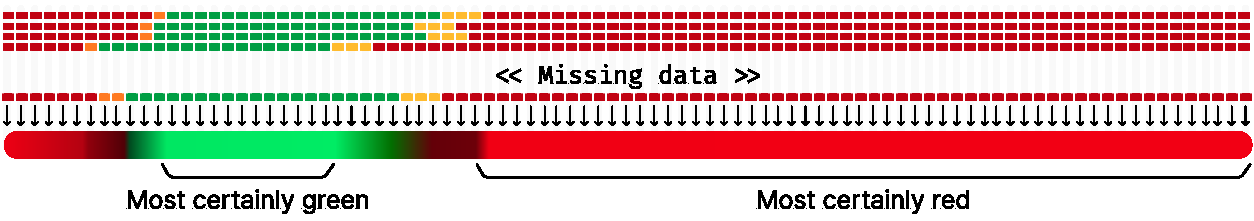
\includegraphics[width=\linewidth]{images/prediction.pdf}
\caption{Probabilistic method of traffic light prediction with cycle stacking.}
\label{fig:prediction}
\end{figure}

Probabilistic methods have been proposed by Protschky et al. (2014) \cite{protschky_extensive_2014, protschky_adaptive_2014} and also Pape (2012) \cite{pape_untersuchung_2012}. The idea of these methods is as follows. Since a fixed per-traffic-light cycle length is mandatory even with fully adaptive traffic light programs \cite{protschky_extensive_2014}, the recorded history can be convolved into a stack of cycles as highlighted in \Cref{fig:prediction}. Then, the probability of "green" and "red" is determined for each second in the prediction vector depending on the prevalence of the predicted color at this specific second in previous cycles.

As discussed earlier, Protschky et al. (2014) \cite{protschky_extensive_2014, protschky_adaptive_2014} have shown that this method is not only scalable but also works well in the presence of high latencies or data losses of real-time traffic light messages. Since the adaptive component is represented as a probability, the speed advisory can focus on certain parts of the prediction, counteracting the adaptive behavior. To traffic adaptive signal timing, this kind of prediction algorithm reacts by blurring out certain parts of the prediction. Thus, as discussed by Otto et al. (2023) \cite{otto_framework_2023}, with a highly adaptive traffic light, one challenge is that the green and red predicted phases can become indistinguishable from each other. In case a target speed is calculated, the speed advisory algorithm must decide which parts of the prediction are considered safe enough. If no parts of the prediction exceed the defined certainty threshold, no speed advisory can be calculated. This is shown by Mahler et al. (2012) \cite{mahler_reducing_2012}, who developed an optimization method for calculating the optimal speed with an uncertain prediction. One challenge of this approach is that, as adaptability increases, it tends to converge more towards the midpoint of the green phase. Following the speed recommendation may result in the vehicle not reaching the traffic light precisely on time but rather with some delay.

Self-adaptive prediction models address this issue very differently. Through continually adapting the prediction to the observed real-time state, the prediction gets more accurate as it approaches the actual time of switching. Bodenheimer et al. (2014 -- 2015) \cite{bodenheimer_enabling_2014, bodenheimer_glosa_2015} were the first to propose such an approach through a graph-based method. This method observes the ingress directions at an intersection node and reconstructs the relation between the clearance timing of each direction. Schneegans et al. (2023) \cite{schneegans_prediction_2023} also demonstrate the possibility of utilizing machine learning models for this process. Here, the idea is to utilize a sequence prediction model trained on prerecorded timing data from a specific traffic light. Both models have the advantage that the predicted residual time readjusts toward the actual observed data at the expense of stretching or shortening the predicted residual time.

As Stahlmann et al. (2018) \cite{stahlmann_exploring_2018} point out, this stretching and shortening can also be seen as a major disadvantage of this approach. Since repeated adjustments to the prediction during the intersection approach negatively impact usability, there is a clear tradeoff between the prediction's accuracy and temporal stability. The increased computational complexity of the presented models is also a factor that may negatively impact the prediction algorithm's scalability toward multiple thousand signals. There is currently no evidence supporting the scalability on a large scale as opposed to probabilistic approaches \cite{protschky_extensive_2014, protschky_adaptive_2014}. Furthermore, while the probabilistic approach is intrinsically robust to incomplete data and can drop individual cycles, error robustness is another factor to consider in the evaluation of self-adaptive models. These challenges must be addressed in order to employ such a model in practice. Most importantly, however, the traffic light data must arrive in time for the self-adaption to happen. Thus, self-adaptive prediction methods can only be employed when the traffic light data arrives with a low latency. In a situation such as reported by Protschky et al. (2014) \cite{protschky_extensive_2014, protschky_adaptive_2014} where traffic light messages may arrive with a delay of over 10 minutes, such models are likely not a good option.

To resolve the dispute between probabilistic and self-adaptive methods, an overarching question is how many traffic lights are, in fact, traffic-adaptive and to what extent they are adaptive. This question must be answered to determine the likelihood that users will encounter inaccurate predictions at intersections. Looking at related work, various studies report different levels of adaptiveness. Cai et al. (2009) \cite{cai_adaptive_2009} were the first to report that "most" signals in their context are traffic-adaptive. Concrete numbers were presented by Bodenheimer et al. (2014) \cite{bodenheimer_enabling_2014}, who reported that 95\% of signals in Hamburg are adaptive, with 73\% being fully or semi-adaptive in the ten largest German cities. Fakler et al. (2014) \cite{fakler_structures_2014} also found a high proportion of traffic-actuated control systems in German cities with over 50,000 inhabitants. Schneegans et al. (2022) \cite{scheegans_exploiting_2022} and Heckmann et al. (2023) \cite{heckmann_stage_2023} further support the conclusion that most traffic lights are operated by traffic-adaptive controls. Hao et al. (2019) \cite{hao_eco-approach_2019} noted the widespread deployment of actuated traffic light controllers in the US, while Avatefipour and Sadry (2019) \cite{avatefipour_traffic_2018} found that fixed timing is more prevalent in Malaysia. Grumert and Pereira (2022) \cite{grumert_heads-up_2022} observed that 70\% of signals in Sweden are adaptive. However, there are also contradictory statements, such as Olaverri-Monreal et al. (2018) \cite{olaverri-monreal_implementation_2018} reporting that adaptive timing is only implemented in a small number of road networks, and the majority of urban areas still use pre-timed control systems.

It must be considered that the reported proportions of adaptive traffic lights are often not verifiable through external sources. For example, in a work by Bodenheimer et al. (2014) \cite{bodenheimer_enabling_2014}, which mentions 95\% adaptive traffic lights, it was only clarified upon inquiry that these results were based on a survey conducted by a service provider on behalf of Audi. Nonetheless, the main findings seem to align with the distribution reported by Hamburg's authorities, which lies at 90.7\% (1570 from 1731) of control programs capable of traffic-adaptiveness. However, this does not necessarily mean that all 90.7\% of adaptive traffic lights also express adaptive switching behavior. In theory, the capability can be unused or only expressed in minor shifts, which would result in a less problematic impact on the prediction, as suggested by the reported percentages. Currently, there is no study that investigates the types of traffic light adaptiveness observed in the real world and the implications on prediction methods.

\begin{Summary}[Summary of Research Gap]
Many works focus on decentralized data transmission, which is currently not available for cyclist applications. At the moment, cyclist applications of traffic light information services require a centralized traffic light data platform. Most centralized platforms appear to retransmit SPaT messages generated at the intersection controller level. Here, the residual time prediction in SPaT messages can be directly used for a speed advisory application. However, in some cases, SPaT messages may not be available or arrive too late, requiring an own prediction method. Using a probabilistic prediction method seems to be a promising option to implement the traffic light prediction. This approach has already proven effective in the context of centralized systems, as opposed to self-adaptive prediction methods. Whether self-adaptive models can contribute to an enhanced traffic light prediction is subject to the completeness and recency of traffic light data, but also the tradeoff between temporal stability and prediction accuracy. To study this relation further, a direct analysis of traffic light data is required to determine how many traffic lights actually exhibit dynamic behavior and the extent of their dynamism. However, such a study has not yet been conducted. Conclusions regarding the extent to which the dynamism of traffic lights may pose a motivation for self-adaptive prediction systems are, therefore, not definitively established. This constitutes an important research gap.
\end{Summary}

\section{Concept}\label{sec:signal-prediction}

We will conduct two steps to address the described research gaps. First, we will design a prediction infrastructure with the available data foundations in Hamburg. Specifically, we will focus on the chain of information from the traffic lights to the cyclist and identify issues in the data transmission that require further consideration. Since our data infrastructure will also be bound to delays and losses in the traffic light messages, we will have to find a prediction method designed to be robust against these issues while being extensible to other cities and highly scalable. We employ the field-tested prediction algorithm proposed by Pape (2012) \cite{pape_untersuchung_2012} and Protschky et al. (2014) \cite{protschky_extensive_2014, protschky_adaptive_2014} that incorporates all desired capabilities, but have to establish a robust data infrastructure around the prediction algorithm that will provide the foundation for our mobile application.

Finally, we address the need for more research on traffic light adaptiveness and predictability. We analyze how suitable the prediction algorithm is for our scenario based on the large-scale evaluation of the traffic light data. We design and evaluate two novel metrics that allow us to measure and systematize types of adaptivity in traffic lights and how they influence traffic light prediction. Based on these concepts, the goal is not only to develop a functional prediction infrastructure but also to learn more about the facets of traffic light prediction in a large-scale urban environment, thus addressing the identified research gap.

\subsection{Prediction Infrastructure}

Providing a traffic light prediction service for users of a cyclist application is strongly linked to the ability to obtain the corresponding real-time data. Although Hamburg provides RSUs at intersections that send SPaT messages, this data source is excluded from further consideration due to its current incompatibility with a smartphone application. Utilizing the control program engineering plans directly for prediction, even if these were accessible, is also not an option for 90.7\% of non-fixed traffic lights in Hamburg. Fortunately, Hamburg provides a centralized traffic light data broker service, the Traffic Light Data (TLD) platform, that provides the necessary real-time data. This platform will be considered the foundation for this work.

\begin{figure}[t]
\centering
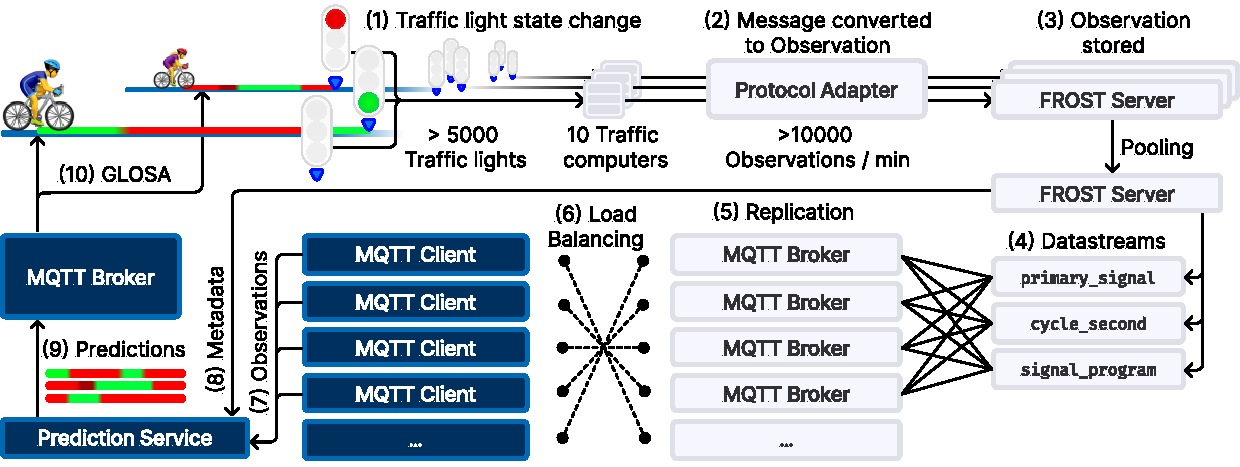
\includegraphics[width=\linewidth]{images/traffic-light-data-infrastructure.pdf}
\caption{Designed traffic light data adapter for Hamburg's Traffic Lights Data platform.}
\label{fig:traffic-light-data-infrastructure}
\end{figure}

It is crucial to understand the type of information provided by the centralized data broker. As mentioned previously, the Traffic Light Data broker does not directly provide SPaT messages, and also no residual time until the next phase change. Instead, the traffic light state messages are provided as observations of the external traffic light state. Specifically, the state messages are provided in the OGC SensorThings\footnote{\url{https://www.ogc.org/standard/sensorthings/}} "Observation" format. Each time the signal changes its color, switches to another program, or restarts a cycle, an Observation is generated and distributed on a corresponding information channel via an MQTT broker. The prediction algorithm has to ingest this data and generate a prediction of the future states.

Until the traffic light state messages arrive at the prediction service, they are translated and shifted multiple times between various data brokers. \Cref{fig:traffic-light-data-infrastructure} highlights Hamburg's data pipeline. First, the state messages are sent in a controller-specific format, such as OCIT\footnote{\url{https://www.ocit.org/de/ocit/schnittstellen/}}, to one of ten traffic computers (1). Then, the messages are converted to Observations (2) and sent to a corresponding SensorThings server. From there, a centralized SensorThings server collects all Observations (3), which are associated with a specific type of "Datastream" encapsulating the type of Observation: \texttt{primary\_signal} for traffic light color, \texttt{cycle\_second} for cycle timing, and \texttt{signal\_program} for program change (4). Finally, the messages are redistributed across an autoscaled cluster of SensorThings MQTT brokers (5). 

From there, the prediction service connects to the broker endpoint to ingest all Observation messages. To reduce the load on each individual MQTT broker, the prediction service utilizes multiple MQTT clients with individual TCP connections (6). The collected Observations (7) are combined, knowing which Observation is associated with which Datastream and which traffic light is represented by a "Thing" (8). This allows the prediction service to record the traffic light history and employ a probabilistic prediction method proposed by Pape (2012) \cite{pape_untersuchung_2012} and Protschky et al. (2014) \cite{protschky_extensive_2014, protschky_adaptive_2014} (9). Every 60 seconds, a new prediction of 180 seconds into the future is generated for each traffic light and distributed to the smartphone app via MQTT (10). Each smartphone app is subscribed to the MQTT topic of the upcoming traffic light, meaning that predictions are automatically updated on the client side.

\begin{figure}[t]
\centering
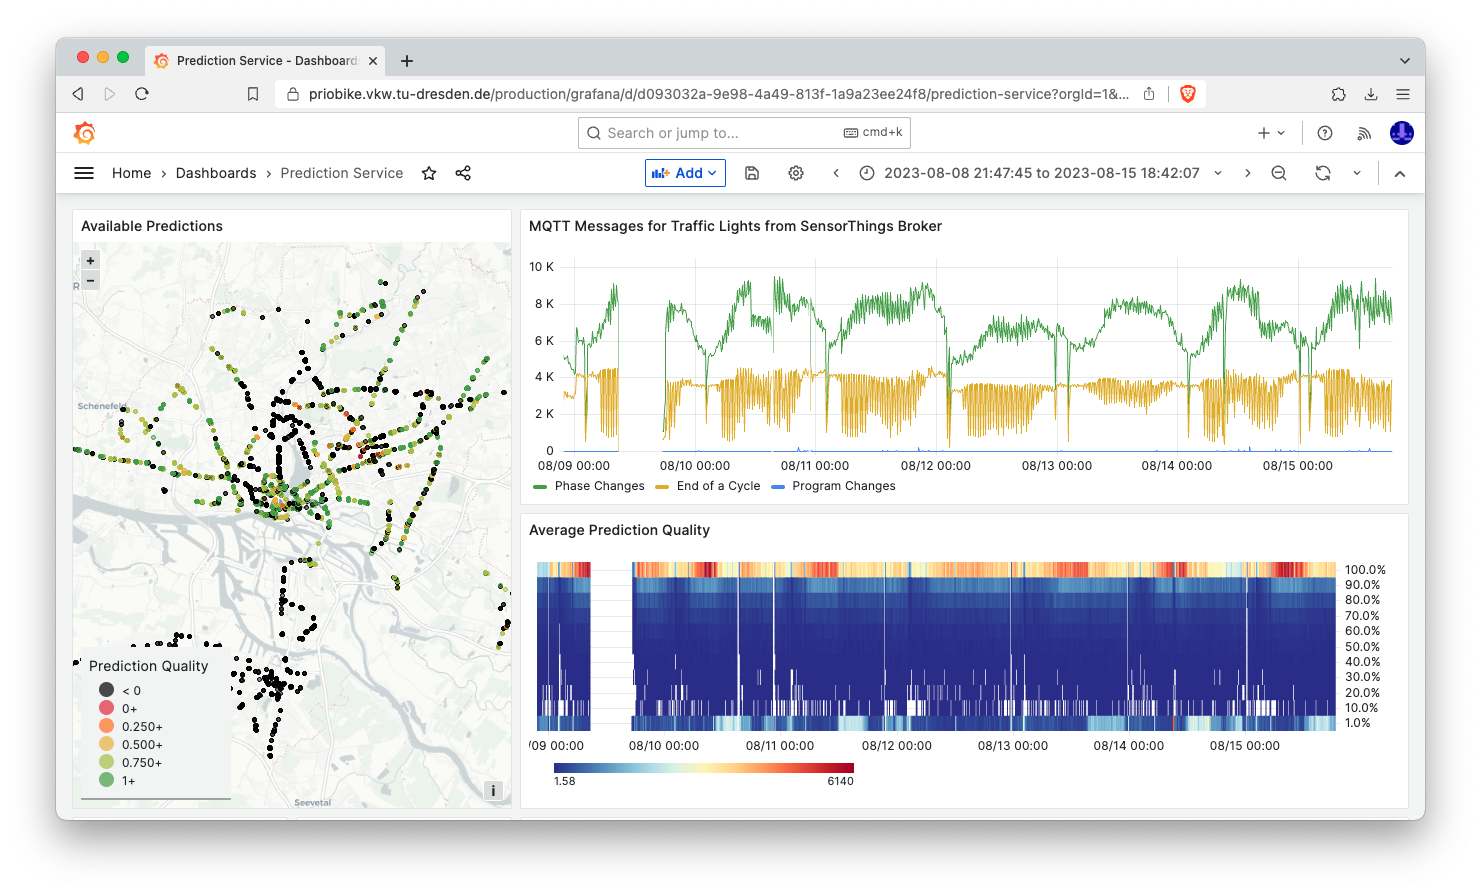
\includegraphics[width=\linewidth]{images/monitoring-screenshot.png}
\caption{Screenshot of the developed monitoring solution. The dashboard displays the current spatial availability and quality of predictions, as well as a timeline for the ingress data and the prediction quality.}
\label{fig:monitoring-screenshot}
\end{figure}

Each time a state message is shifted along the presented chain of information, it introduces a delay and a possible point of failure. As a consequence, the prediction service must be robust against delayed or missing state messages. However, these issues are not evenly distributed across all traffic lights. They may arise in specific areas in the city or from time to time. Thus, it is also important to monitor this behavior and identify and address systematic issues in the traffic light data infrastructure. As a foundation, as shown in \Cref{fig:monitoring-screenshot}, a monitoring system was implemented that highlights data outages across the city and along a timeline.

In addition to these coarse-grained methods, another error-detection is implemented that detects missing state messages for traffic lights. The designed detection makes use of the shifting pattern red-redamber-green-amber and red-green. Transitions between phases are checked against these allowed transitions. If an illegal transition occurs, the currently recorded cycle is discarded. This makes use of the probabilistic prediction method's robustness against missing cycles.

\begin{figure}[htbp]
\centering
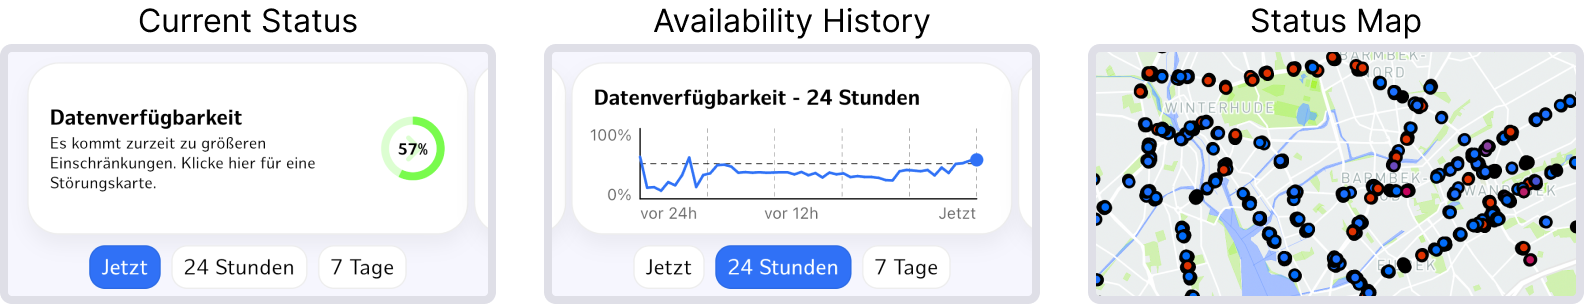
\includegraphics[width=\linewidth]{images/home-view-prediction-quality.png}
\caption{Prediction quality visualized in the GLOSA app for enhanced explainability.}
\label{fig:home-view-prediction-quality}
\end{figure}

Not all traffic lights in Hamburg are available for prediction. Those who are available may occasionally lose data, which error detection can partially address. Another important factor, however, is the user's perspective on the data availability. Since a degraded prediction availability will also negatively impact usability, some ideas must be found that mitigate potential disappointments on the user side. One idea implemented in the GLOSA app is increasing the explainability of the prediction system. The existing monitoring infrastructure is extended such that users can also access information about the current availability. Through the app, users can inform themselves about the current percentage of available predictions and the spatial distribution of good and bad predictions on the map. The resulting user interface shown in \Cref{fig:home-view-prediction-quality} is intended to allow users to identify faults at an early stage and then switch to an alternative app, avoiding frustration caused by missing or incorrect predictions.

\subsection{Predictability Analysis}

Considering the potential traffic-adaptive behavior of traffic lights, it is clear that we cannot predict each one equally well. Understanding the quantity and implications of traffic-adaptive behavior on the prediction method is crucial. However, previous work has only dealt superficially with this issue. There are no precise criteria or metrics that can be used to decide how well traffic lights are predictable and which prediction method is the most suitable. In this section, we will derive such criteria and develop a systematic model to determine how suitable our prediction model is. With the real-time data available from the traffic lights in Hamburg, we can then implement our process model and derive findings on the actual predictability of traffic lights.

The predictability of traffic lights depends on the stability of patterns in the switching behavior. Only if there are reoccurring patterns, the traffic light can be predicted. Vice versa, a highly spontaneous and thus unstable switching behavior is related to low predictability. Assuming alignment of a traffic light's switching behavior with the cycle length \cite{protschky_extensive_2014}, one option to measure the switching behavior's instability is counting the seconds differing between two cycles $C_1$ and $C_2$ with the length $l_1$ and $l_2$ in the recorded history. As a result, we obtain a cycle-dependent instability metric measured in seconds of discrepancy between cycles:

\begin{equation} \text{Cycle-Dependent Instability}(C_1, C_2) =  \sum_{i=0}^{\max(l_1, l_2)-1} \left\{
\begin{array}{ll}
1 & \text{if } i \geq l_1 \text{ or } i \geq l_2 \\
1 & \text{if } C_1[i] \neq C_2[i] \\
0 & \text{otherwise}
\end{array} \right.\end{equation}

One limitation of this metric is that it does not capture reoccurring patterns between green phases that are not aligned with the cycle length. As a result, the time between green phases could be constant but result in a high cycle-dependent instability if the green phases are not aligned relative to the cycle start time. To cope with this issue, a second metric is required that measures the instability independent of the cycle length. 

The additional cycle-independent instability metric is designed as follows. First, the recorded cycles are concatenated into a continuous history $H_{C_1, \dots, C_n}$ of traffic light switching. Then, between every two green phases for which a continuous record is present, the wait time in between is measured and rounded in seconds. As a result, we obtain a list of wait times between green phases. Then, we measure how many \textit{different} waiting times are seen proportionally to the number of all wait times:

\begin{equation}
\text{Cycle-Independent Instability}(H_{C_1, \dots, C_n}) = \frac{\text{\# Different Wait Times}}{\text{\# Total Wait Times}}
\end{equation}

In the extreme case that only one green phase is detected, the metric is set to 1, meaning that no reoccurring pattern was detected. If no green phase is detected, the metric is set to 0, assuming that this represents an easily predictable pattern (always red). Otherwise, if there are more reoccurring green patterns in the wait time, the cycle-independent instability is expected to be close to 0. Here, it doesn't matter whether the reoccurring patterns are aligned with the cycle time or if these revolve after a few cycles. If the variability of waiting times between green phases is high, and thus the number of different wait times, the cycle-independent instability is expected to be close to 1. 

Since the cycle-independent instability, however, does not necessarily capture the amount of shift between green phases and only the uniqueness, it is not entirely better than the cycle-dependent instability metric. Both measures need to be employed in conjunction to determine whether predictable patterns are present.

\begin{figure}[t]
\centering 
\begin{tabular}{|c|c|c|}
\hline
& \footnotesize{\textbf{Low cycle-dependent instability}} & \footnotesize{\textbf{High cycle-dependent instability}} \\
\hline
\rotatebox{90}{\footnotesize{\textbf{\hspace{0.18cm} High cycle-independent instability}}} & B 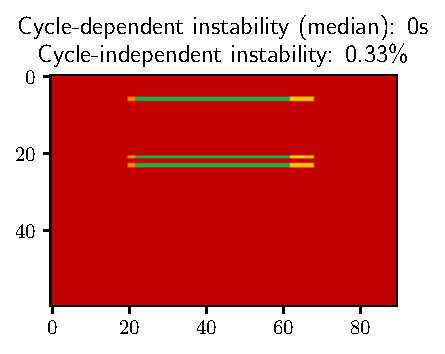
\includegraphics[width=0.42\linewidth]{images/predictability-cycles-1.pdf} & D 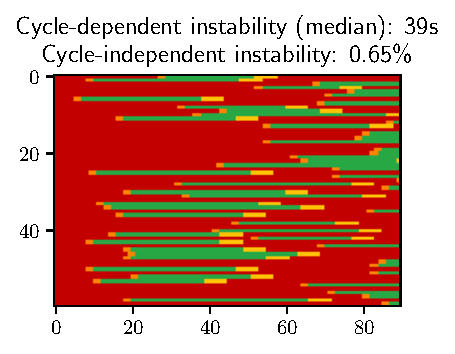
\includegraphics[width=0.42\linewidth]{images/predictability-cycles-2.pdf} \\
\hline
\rotatebox{90}{\footnotesize{\textbf{\hspace{0.18cm} Low cycle-independent instability}}} & A 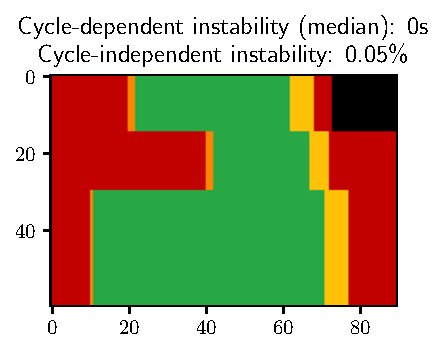
\includegraphics[width=0.42\linewidth]{images/predictability-cycles-3.pdf} & C 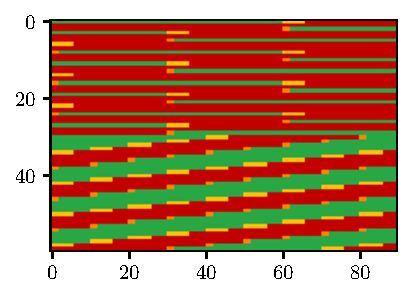
\includegraphics[width=0.42\linewidth]{images/predictability-cycles-4.pdf} \\
\hline
\end{tabular}
\caption{.}
\label{fig:types-of-instability}
\end{figure}

\Cref{fig:types-of-instability} provides a systematic model for the types of instability that can be measured with our two metrics. In case A, the green phases are both aligned with the cycle time and at relatively constant distances from each other. Thus, both the cycle-independent and cycle-dependent instability is low. In case B, the green phase is only occasionally switched upon detection of a vehicle, cyclist, or pedestrian. As a result, the cycle-dependent instability is low since all cycles are very similar to each other. However, since the waiting time between green phases is highly variable, the cycle-independent instability is high. Case C highlights the scenario that is not captured well by the cycle-dependent metric alone. A "staircase" pattern is present, meaning that the green time is shifted in a constant rhythm that is not aligned with the cycle time, resulting in a high cycle-dependent instability but a low cycle-independent instability. Finally, case D contains the least predictable switching behavior, which expresses both cycle-dependent and independent instability. 

Locating traffic lights on this 2-dimensional scale will help us determine which kinds of patterns are present. It also helps us find the number of cases in which our prediction method is inadequate, especially with respect to cases C and D. In general, the more cases are similar to A and B, the better for our chosen probabilistic prediction method. Finally, we can explore these metrics in other dimensions, such as over time in a week, to gain additional insights about predictability.

\begin{Summary}[Summary of Methods]
The designed prediction infrastructure makes use of Hamburg's centralized Traffic Light Data platform and reuses the existing probabilistic prediction method  \cite{pape_untersuchung_2012, protschky_extensive_2014, protschky_adaptive_2014} guaranteeing scalability in addition to robustness to latencies and data errors. Interoperability with platforms without the availability of intersection-controller-level predictions (as with SPaT messages) is also given since the prediction algorithm only relies on the availability of traffic light colors and cycle timing information. Additional measures are implemented that detect and discard erroneous data. Through a monitoring system the prediction quality can be analyzed and systematic issues identified. Information about the prediction availability is forwarded to the user to enhance the explainability of outages. 

In addition to this monitoring system, a predictability analysis is conducted to explore the traffic-adaptiveness of traffic lights. This predictability analysis reuses the established traffic light data infrastructure in Hamburg to record and analyze traffic light cycles. Through a direct measurement of the observed switching patterns a more direct view of the predictability is provided than given in previous studies. The adaptiveness is measured with two metrics in conjunction: the cycle-dependent instability metric incorporating the discrepancy between traffic light cycles and the cycle-independent instability metric that measures the uniqueness between wait times.
\end{Summary}

\section{Results}

The evaluation of the prediction infrastructure is divided into two parts: the assessment of the prediction process and the evaluation of traffic light predictability in Hamburg.

Firstly, we examine how well the prediction system interacts with the Hamburg Traffic Light Data platform and identify potential weaknesses. This involves analyzing the spatial coverage and trends of traffic light predictions over an extended period, utilizing recorded metrics from the implemented monitoring system. We investigate the temporal availability of predictions to understand the number of traffic lights in Hamburg where speed recommendations can be expected. Our findings indicate that the availability is significantly lower than desired. To delve deeper into the reasons for this, we examine the recorded metrics from the implemented monitoring tool, identifying recurring error patterns that suggest systematic issues in the Hamburg data infrastructure. Collaborating with the data platform operators, we draw conclusions about the root causes of these problems and propose potential solutions. To further demonstrate the scalability of the prediction algorithm, we briefly examine the CPU, RAM, and network usage of the prediction service.

The second part of the evaluation focuses on studying traffic adaptability through real-time data. We analyze the day-night cycle of traffic adaptiveness from weekday to weekday, examining how much the green phase of traffic lights fluctuates forward and backward in a cycle, utilizing the developed cycle-dependent instability metric. Additionally, we investigate whether green phases tend to distribute evenly within the cycle or if there are traffic lights with step patterns where the green phase only fluctuates forward or backward. Using a map, we assess whether traffic dependence affects entire intersections with multiple traffic lights as expected or if it also impacts individual traffic lights. These analyses provide insights into estimating the suitability of the designed prediction process and point out intersections at which another prediction method could be a better option.

\begin{table}[b]
    \centering
    \begin{tabular}{@{}l|ccccccccc|r@{}}
        \hline
        \textbf{Lane type} & \multicolumn{9}{c|}{\textbf{Tag according to \texttt{Thing/properties/laneType}}} & $\Sigma$ \\
        \hline
        Car        & $\blacksquare$ & $\blacksquare$ & $\blacksquare$ &   &   & $\blacksquare$ &   &   &   &  9649 \\
        Bus        &   &   & $\blacksquare$ &   &   & $\blacksquare$ & $\blacksquare$ &   & $\blacksquare$ &  1309 \\
        Bike     & $\blacksquare$ &   & $\blacksquare$ & $\blacksquare$ &   &   &   & $\blacksquare$ & $\blacksquare$ &  5477 \\
        Pedestrian &   &   &   &   & $\blacksquare$ &   &   & $\blacksquare$ &   &  6408 \\
        \hline
        $\Sigma$ (unique) & 1509 & 7077 & 217 & 3646 & 6315 & 846 & 234 & 93 & 12 & \\
        \hline
    \end{tabular}
    \caption{Number of individual traffic lights (connections) in the Traffic Lights Data platform, as of Dec 4, 2023.}
    \label{tab:tld-number-of-things}
\end{table}


\subsection{Long-Term Study of Prediction Availability, Quality, and Scalability}

When examining the temporal progression of the prediction, it is crucial to note the continuous increase in the number of traffic lights in the Traffic Lights Data platform. The ID of individual traffic lights (connections) can be utilized to determine the number of intersections, such as \texttt{353\_12} for intersection node 353 and Connection 12. Referring to \Cref{tab:tld-number-of-things}, as of December 2023, there are 19,951 connections distributed across 791 intersection nodes in the system. This constitutes a coverage of 45.7\% (of 1,731) of signalized intersections. During a preliminary examination of traffic lights, two minor errors were identified:

\begin{enumerate}
    \item One of the traffic lights (132\_22) exhibited a duplicated \texttt{cycle\_second} data stream.
    \item Additionally, \texttt{laneType} "16371" was mistakenly assigned to connections 240\_1 and 240\_2. These are not included in \Cref{tab:tld-number-of-things} as they cannot be accurately assigned.
\end{enumerate}

Both issues were traced back to data input errors through communication with operators, and corrective measures have been initiated.

\begin{figure}[t]
    \centering
    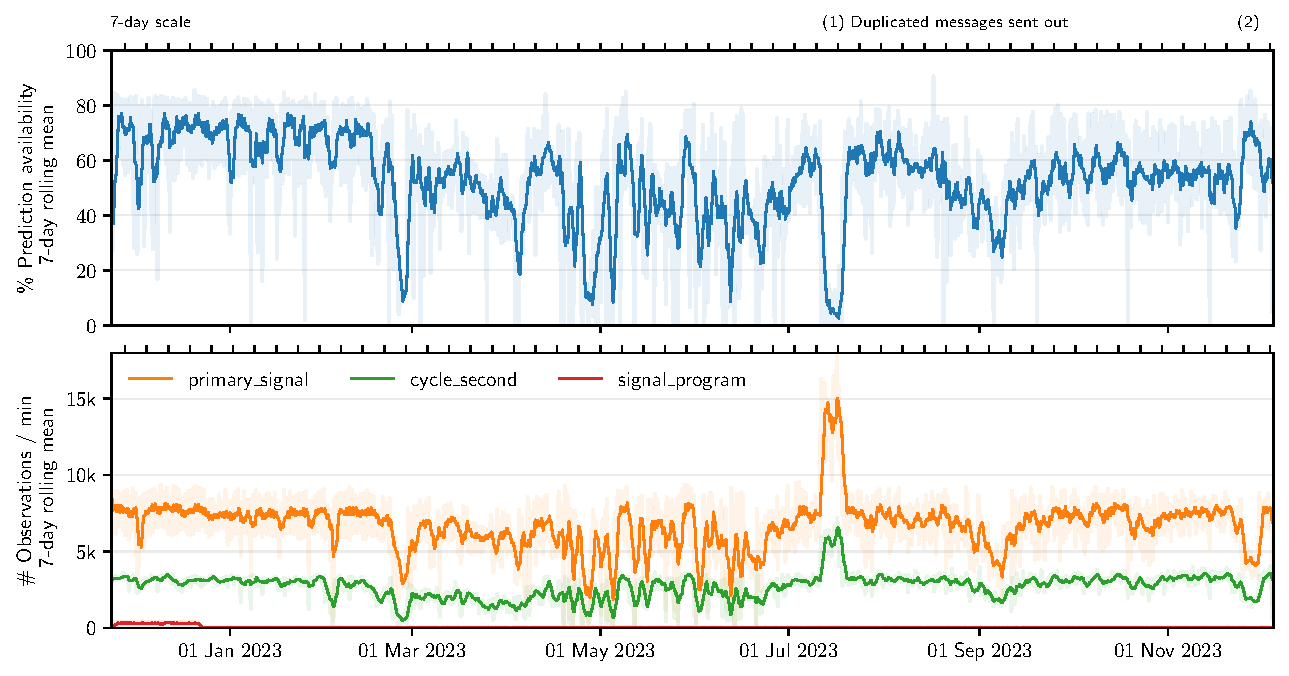
\includegraphics[width=\linewidth]{images/monitoring-availability.pdf}
    \caption{Long-term development of prediction availability.}\label{fig:monitoring-availability}
\end{figure}

As of December 4, 2023, out of the 19,951 traffic lights, 5,477 are designated for use by cyclists and are thus relevant to our bike-GLOSA system. This also includes mixed usage by public transportation, pedestrians, and cars, along with bicycles. Recorded data for these traffic lights, measured over a period of 365 days (December 4, 2022 - December 4, 2023), show an average of 8,532 \texttt{primary\_signal} observations, 3,318 \texttt{cycle\_second} observations, and 27.7 \texttt{program\_change} observations per minute received and processed via MQTT. During this time, the Prediction Service was offline for 75 hours due to planned maintenance or technical issues and online for 8,680 hours, resulting in a calculated 99.14\% uptime. For 5 hours, the status is unclear as the entire VM or only the monitoring was offline. Assuming 80 hours of downtime, we have a 99.08\% uptime. Therefore, it should be noted when interpreting the following metrics that not 100\% of the time period is covered.

The long-term data trend and prediction availability are depicted in \Cref{fig:monitoring-availability}. The prediction availability is calculated by dividing the number of predictions generated per minute by the total number of available connections. In the upper part of the figure, we observe that prediction availability typically fluctuates between 40\% and 80\%, with 100\% never being reached.

The prediction availability varies throughout the day and over the longer recording period. Examining the long-term trend, we notice increased disruptions in prediction availability in the summer of 2023, following an initial period of relatively stable availability. These disruptions stabilize around October 2023 but do not return to the levels seen in the spring of 2023. The disruptions in summer 2023 are primarily attributed to increased maintenance activities on the Traffic Lights Data System. Repeated updates during this period led to a deterioration in data quality. 

For instance, around July 11, 2023 (1), all observations were accidentally sent twice, causing prediction availability to nearly drop to 0\%. This incident represents the most significant observed disruption. One hypothesis for the drastic decline is that the duplicate messages originated from a mirrored system with different latency, arriving at a different time than the originals, invalidating the recorded traffic light switching history. Around November 23, 2023 (2), a feature was tested to exclude malfunctioning traffic lights from the prediction system, leading to a brief increase in relative availability despite a decrease in observations.

\begin{figure}[t]
    \centering
    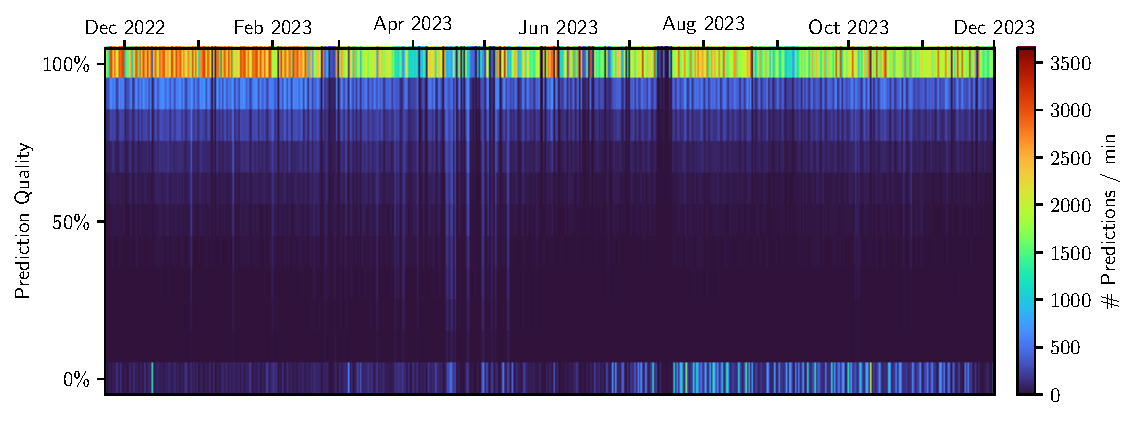
\includegraphics[width=\linewidth]{images/monitoring-long-term-study.pdf}
    \caption{Long-term development of prediction quality.}\label{fig:monitoring-long-term-study}
\end{figure}

Apart from these two exceptional situations, it is evident that prediction availability strongly correlates with the absolute number of messages. The decline in \texttt{signal\_program} observations in December 2022 remains unclear. Without a ground truth and a detailed record of metrics for that period, it is challenging to determine whether only a fraction of the actual program observations arrived at this time or if an excessive number was sent in December 2022.

Furthermore, it is important to note that the analysis in \Cref{fig:monitoring-availability} does not account for the quality of the prediction. Some forecasts are generated and therefore recorded in the displayed availability but have low quality. Since speed recommendations are not displayed to the user when the prediction quality is below 50\%, the actual availability of speed recommendations is always lower than the prediction availability.

The quality of the predictions is depicted more precisely in \Cref{fig:monitoring-long-term-study}. It is measured through a continuous comparison of the prediction with the actual incoming data. If every second in the prediction vector aligns with the running cycle, the prediction quality is calculated as 100\%. If no seconds align, this results in 0\% prediction quality. The running cycle is not incorporated into the prediction vector yet at the time of prediction quality calculation, ensuring that no running information sinks into the calculated prediction quality. In the current implementation of the prediction procedure, there is also a prediction quality of -1, generated when real-time validation data is no longer available for an extended period of time. In \Cref{fig:monitoring-long-term-study}, this is mapped as a prediction with 0\% quality.

Examining the long-term trend initially reveals a similar pattern in prediction availability at 100\% quality compared to \Cref{fig:monitoring-availability}. Notably, there is a significant dip around July 11, 2023, due to the duplicated observations issue and a general decrease in availability throughout the year 2023. Furthermore, the prediction quality appears dichotomous: only a few predictions fall within the intermediate 10\% to 90\% quality range. If interpreted as an accuracy metric, most predictions seem to be precise to a few seconds. 

Nonetheless, an increase in predictions with 0\% quality has been observed since around July 2023. As the prediction algorithm generates predictions only when real-time traffic light data were available at an earlier time, this suggests intermittent data failures. These failures can be normal, such as during the nightly shutdown of a traffic light, or unintended if they occur irregularly. Since the latter would indicate a systematic issue in the data infrastructure, it is worthwhile to take a closer look at the data failures.

\begin{figure}[t]
    \centering
    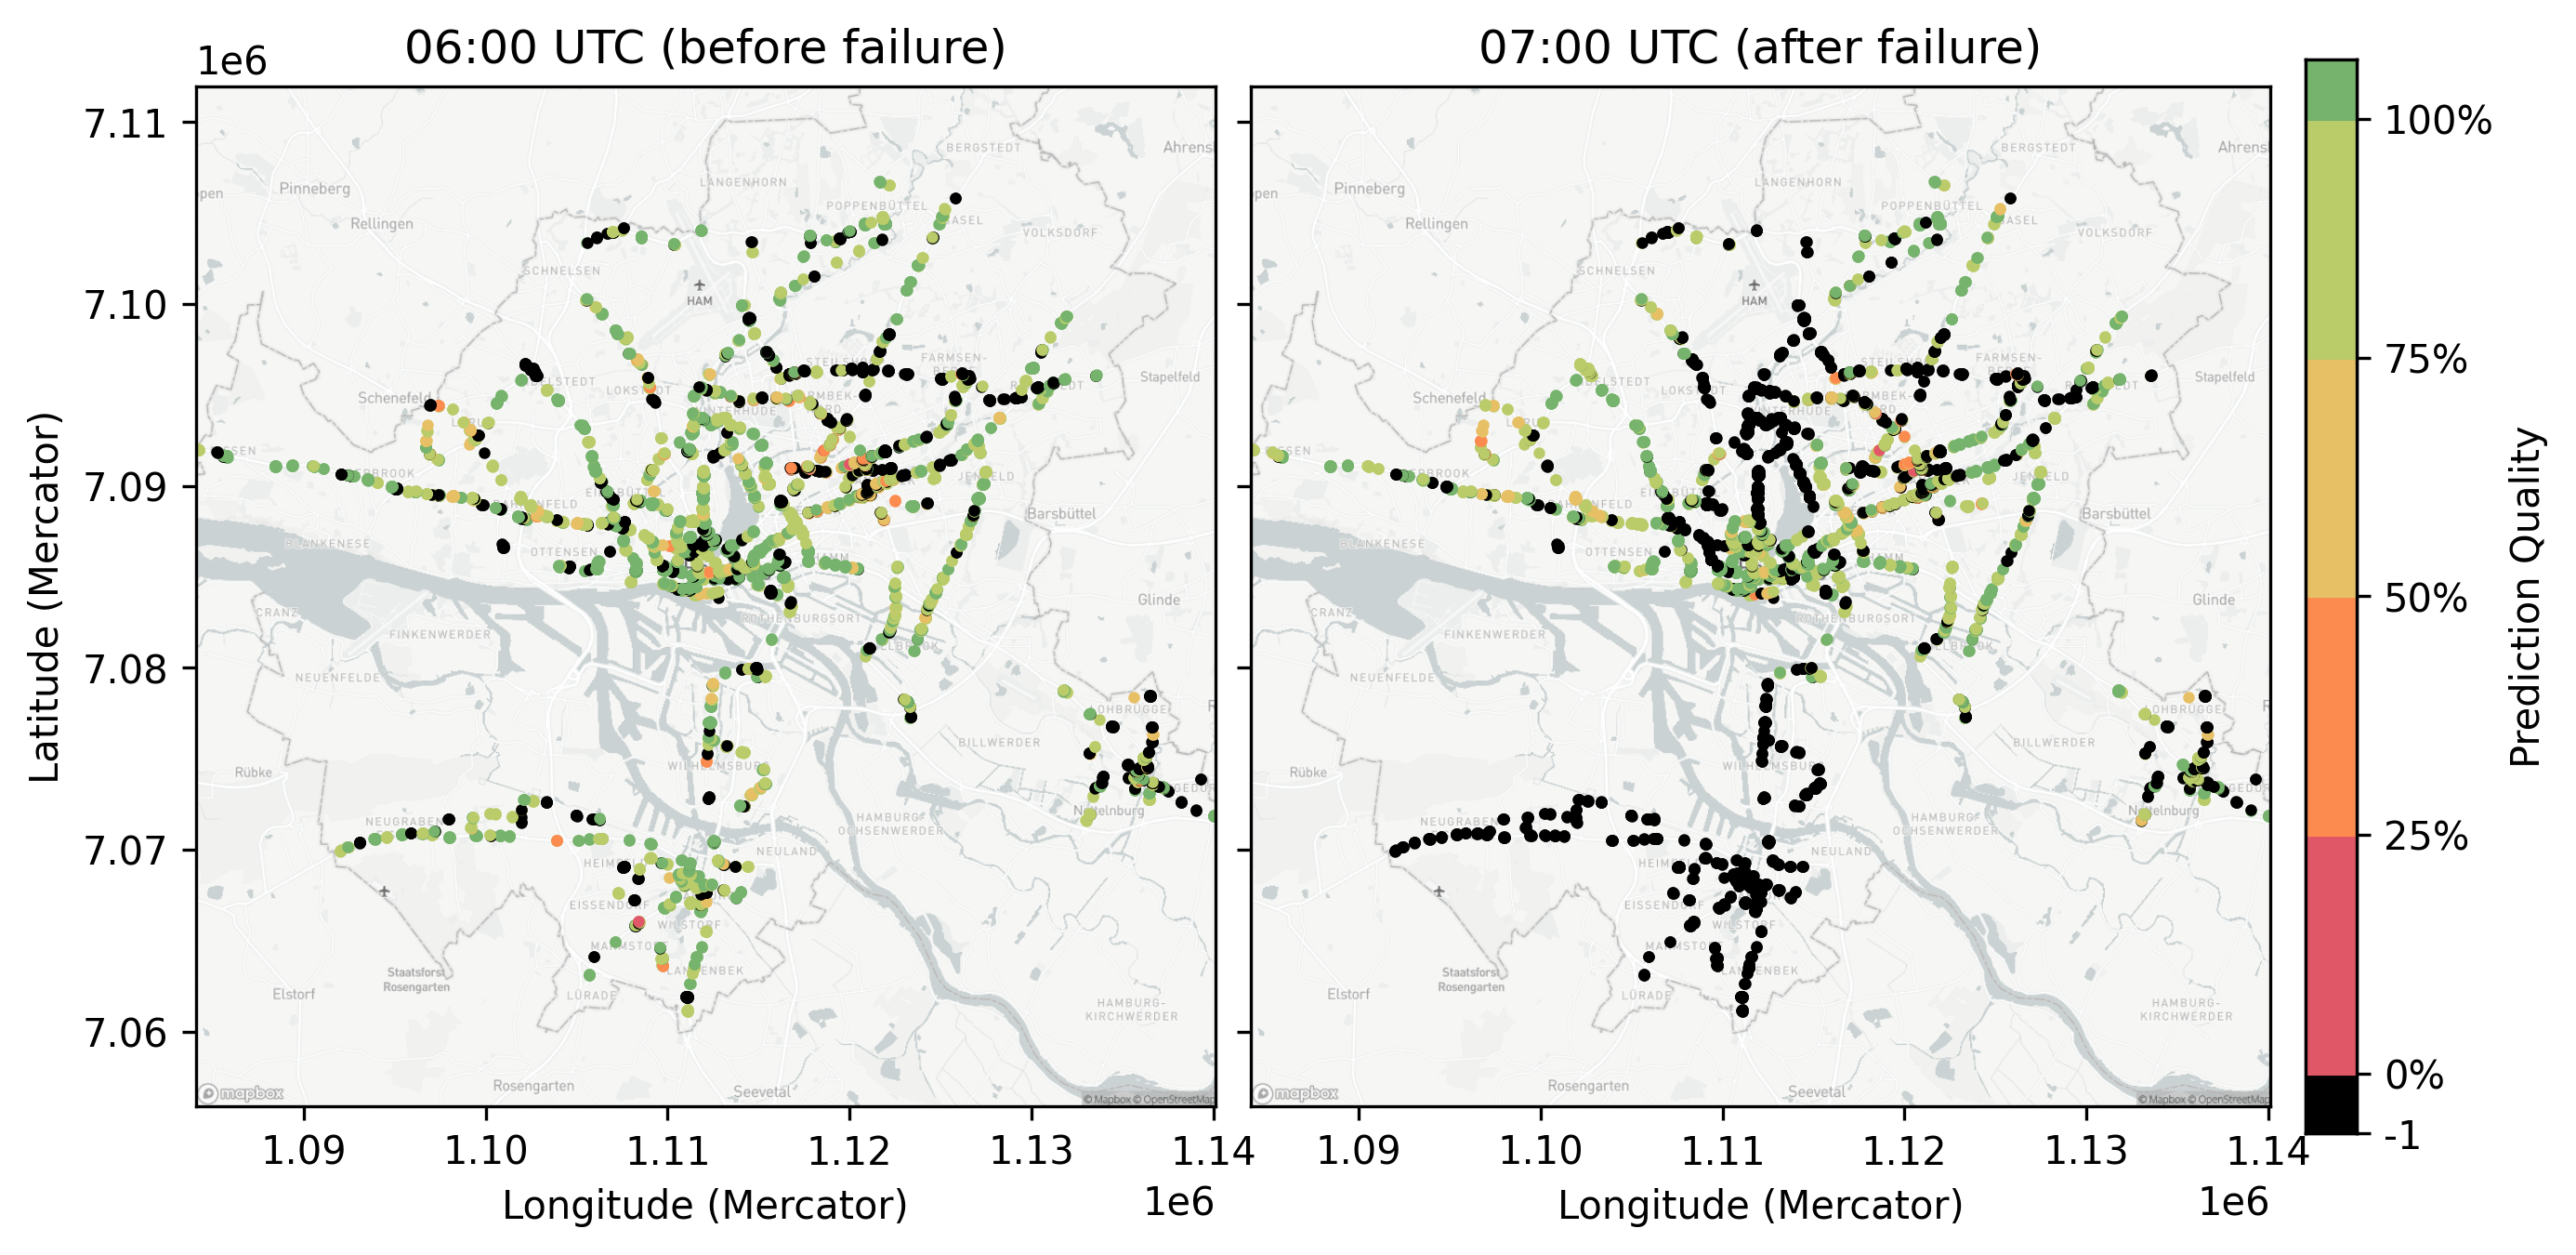
\includegraphics[width=\linewidth]{images/monitoring-before-after-failure.png}
    \caption{Before and after traffic computer failure on Oct 11, 2023.}\label{fig:monitoring-failure}
\end{figure}

An arbitrarily chosen example of such a data failure is illustrated in \Cref{fig:monitoring-failure}. Two distinct error patterns are apparent: failures of individual traffic lights (on the left and right) and failures or impairments affecting entire city districts (on the right only).

Let's examine the failures of individual traffic lights more closely. Collaborating with the operators of the Traffic Lights Data platform, our monitoring identified 61 intersections and 80 individual connections experiencing persistent issues, rendering them unable to transmit data. In at least 30 cases, a connection was associated with an unsignaled road crossing, or the connection was no longer present. Among 22 nodes, traffic lights utilized the OCIT protocol, which is, as of December 2023, unsupported by the Traffic Lights Data platform. For 19 nodes, the observed failures are presumed to be construction-related, with this confirmed in three additional cases. In 16 instances, outdated intersection topologies or georeferences were identified. The identified traffic lights were subsequently excluded from the forecasting system using an exclude list, with the option to reintegrate them later.

Turning our attention to failures affecting entire city districts, \Cref{fig:monitoring-failure} demonstrates their relatively spontaneous occurrence. This type of failure poses a more significant challenge than individual node or connection failures since thousands of predictions are abruptly invalidated. Therefore, it is crucial to precisely identify the origin of this problem.

\begin{figure}[t]
    \centering
    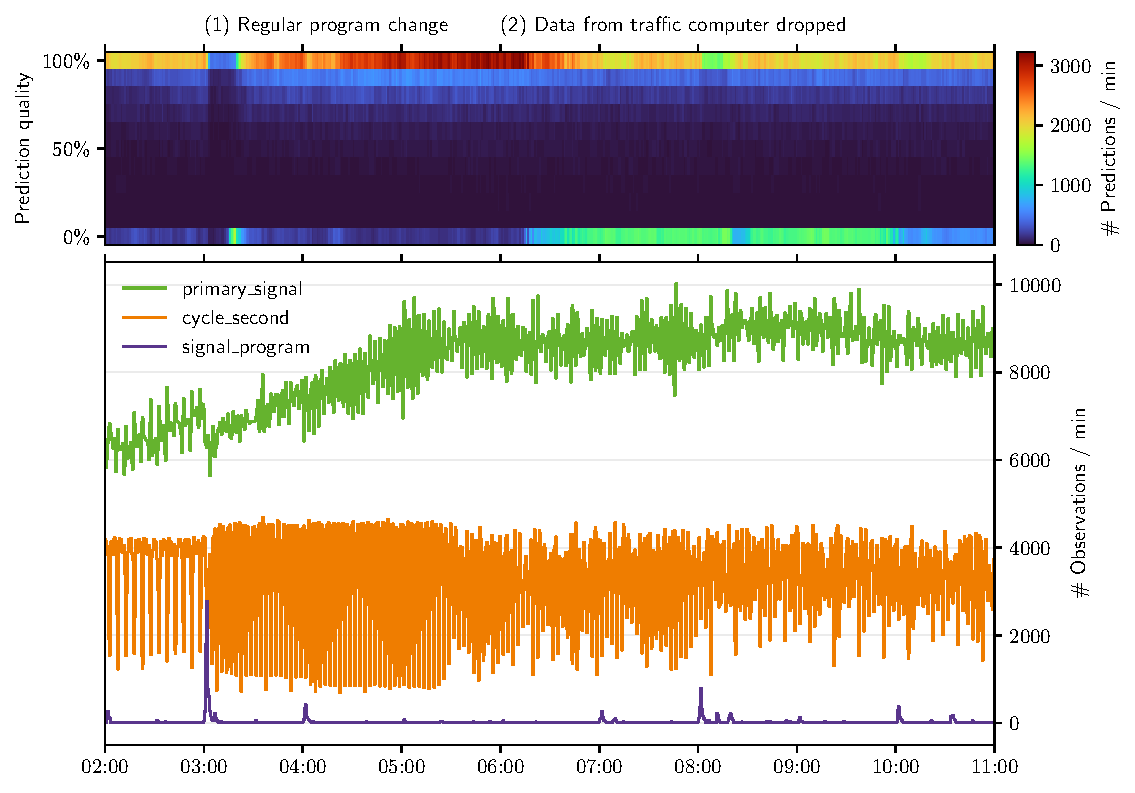
\includegraphics[width=\linewidth]{images/monitoring-failure.pdf}
    \caption{Monitored metrics during traffic computer failure on Oct 11, 2023.}\label{fig:monitoring-failure}
\end{figure}

To better understand the occurrence of such a failure, let's examine the daily course of the above failure scenario, as depicted in Figure \ref{fig:monitoring-failure}. At 3:00 AM UTC, within the timeline of \texttt{signal\_program} observations, we observe that many traffic lights switch their programs. This could, for instance, represent the morning program of the weekly automation of the traffic lights being scheduled.

Simultaneously, the availability and quality of the predictions briefly decline (1). This can be explained by the fact that the prediction algorithm continues to forecast the old pattern from the previous program for a certain period, only synchronizing with the new program after approximately 15 minutes. This flaw in the implementation of the prediction algorithm is known and should be addressed by incorporating program observations into the prediction.

Following this brief decline, the best prediction quality is achieved around 6:00 AM UTC, just before it suddenly and persistently collapses across multiple districts. The fact that these declines are reflected in specific districts strongly suggests that this issue can be traced back to specific traffic controllers, each generating observations for one or more districts. 

Once this observation was communicated to the operators of the Traffic Lights Data platform, it was identified that this problem is indeed associated with certain traffic controllers. The increasing load throughout the day due to rising traffic triggering more green phases causes the message queues of the MQTT brokers at the traffic controllers to fill up. Ultimately, this results in the traffic controllers either not sending messages at all, dropping individual messages, or transmitting them with significant delays.

\begin{figure}[t]
    \centering
    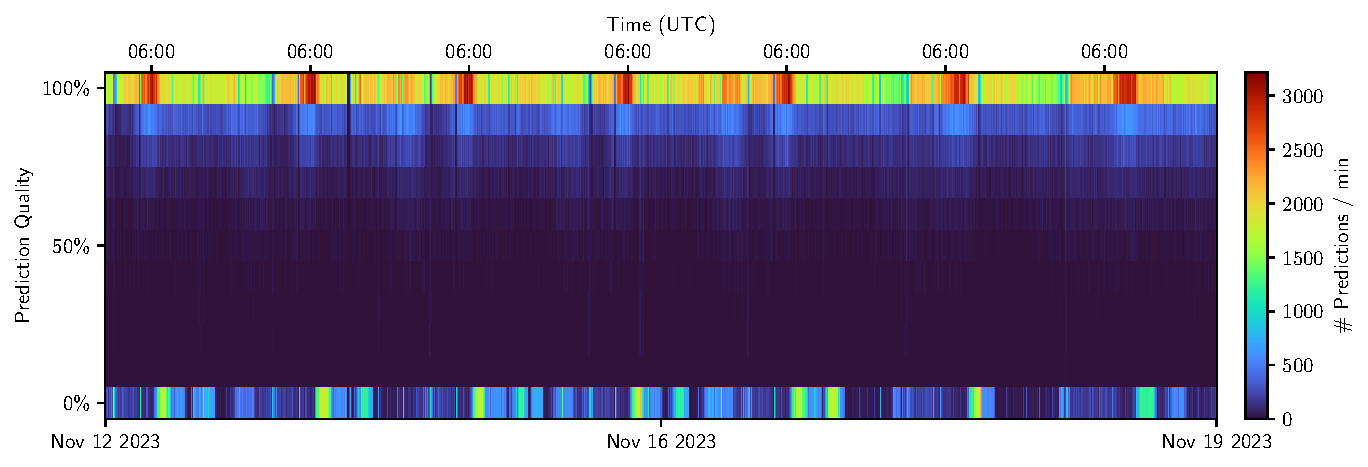
\includegraphics[width=\linewidth]{images/monitoring-7-days.pdf}
    \caption{Reoccurring traffic computer failures after 6:00 UTC.}\label{fig:monitoring-7-days}
\end{figure}

In the weekly progression illustrated in \Cref{fig:monitoring-7-days}, it is evident that this situation repeats almost daily at the same time. Only on Saturdays and Sundays does the issue manifest later, around 7:00 - 8:00 AM UTC, due to reduced and delayed traffic leading to fewer green phases.

Upon identifying the root cause, the operators initiated appropriate fixes related to the MQTT queues of the traffic controllers. Simultaneously, an additional exclusion list of intersection nodes was created, preliminarily exempting them from the prediction until the issue was resolved. This involves a total of 584 intersections connected to three specific traffic controllers. The identities of which traffic controllers specifically were affected must remain confidential—refer to \cite{neuner_leitfaden_2020} for more details.

Another analytical approach involves examining how many cycles were discarded due to irregular consecutive signal sequences. This analysis provides further insights into whether isolated messages are lost or if observations from operational traffic lights consistently reach their destination.

\begin{figure}
    \centering
    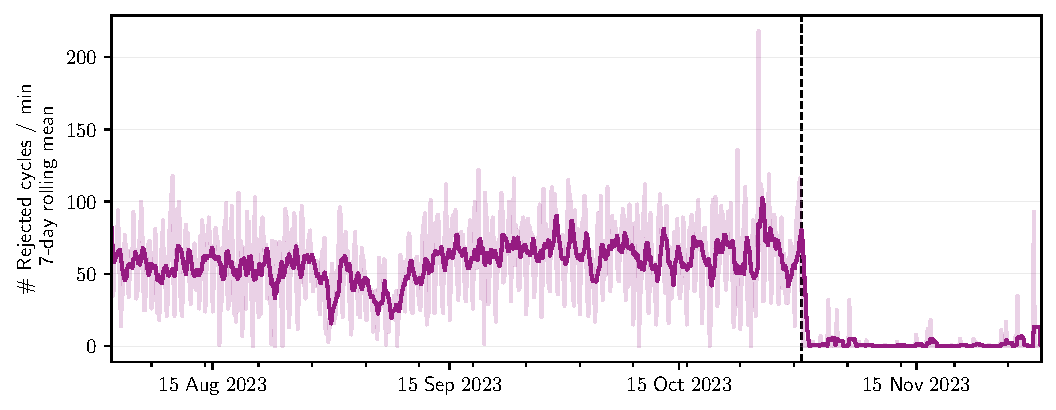
\includegraphics[width=\linewidth]{images/monitoring-rejected-cycles.pdf}
    \caption{Cycles rejected due to out-of-order phase sequence.}\label{fig:monitoring-rejected-cycles}
\end{figure}

The analysis is depicted in \Cref{fig:monitoring-rejected-cycles}. Due to the delayed implementation of error detection in the prediction system, only recorded data from August 1, 2023, onward is available. Nevertheless, a remarkable improvement is evident. On October 31 at 6:40 AM local time, the number of rejected cycles suddenly dropped to 0, with only sporadic peaks. The specific modification made to the Traffic Lights Data System at that time is unknown.

Previously, between 25 and 125 cycles were rejected every minute. Assuming a cycle length of 90 seconds and considering one cycle per connection, this could affect up to 200 connections. However, this had no noticeable impact on the measured forecast quality, as observed in \Cref{fig:monitoring-long-term-study}. One possible explanation is the resilience of the prediction algorithm to individual missing cycles. Another explanation could be the resolution of specific connections that frequently sent consecutive \texttt{cycle\_second} observations, disproportionately generating faulty cycles. The existence of such traffic lights has been previously confirmed through real-time data observations.

Finally, let's review the scalability of the prediction algorithm. For the prediction service implemented in Java, running as a container on the deployment since December 2022, load metrics have been recorded using Cadvisor. This measurement period progressed until May 2023.

\begin{figure}[htbp]
    \centering
    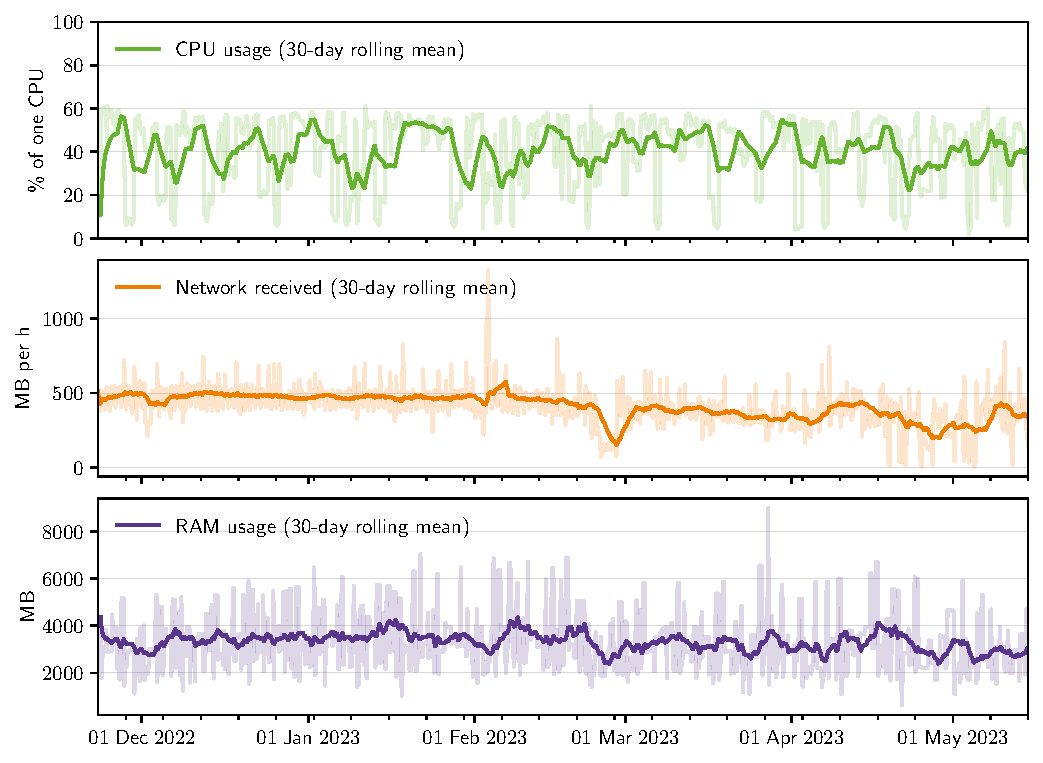
\includegraphics[width=\linewidth]{images/monitoring-prediction-service-load.pdf}
    \caption{Cadvisor statistics for prediction service.}\label{fig:monitoring-prediction-service-load}
\end{figure}

The service was measured on a TU Dresden Enterprise VM with 6 CPU cores. To calculate the percentage utilization of the prediction service on the CPU cores, CPU time was measured. In this context, the service consumes approximately 60\% of the CPU time of a single CPU, translating to around 10\% of the total possible computing capacity when considering 6 CPUs. Both network usage and RAM consumption are also within acceptable limits.

To interpret these numbers, it should be noted that the prediction service encompasses all functionalities required for forecasting, including the handling of all real-time traffic light data ingestion. There is surely potential to further optimize the performance and scalability. However, optimizations in terms of performance are currently not required, as the service appears to scale well. 

For deploying the prediction service across additional cities, adding more VMs into the deployment and, potentially, another MQTT broker for prediction transmission should be sufficient. Allowing the smartphones to connect to the correct broker in the case of a distributed prediction MQTT broker infrastructure should be trivial, e.g., through sending this mapping along the matched traffic lights along the route. Currently, only the network ingress direction could be considered a bottleneck, although it also provides much more headroom.

\subsection{Study of Traffic-Adaptivity in Hamburg}

In the previous section, we found that many traffic lights, in case they send enough data, can be accurately predicted based on the quality metric of our prediction algorithm. The selected algorithm not only appears to scale well but also surprisingly performs effectively with the reported high number of traffic-dependent traffic light systems in Hamburg. This observation contrasts with previous studies that had suggested the opposite.

It is worth noting that our analysis has so far focused only on bicycle traffic lights, providing only a partial picture. Therefore, our next step is to examine the predictability of all traffic lights in Hamburg in a broader context. This analysis aims to gain deeper insights into traffic light schedules and, ultimately, to identify areas for future optimizations of current prediction systems.

To conduct these evaluations, real-time data was recorded for approximately four weeks. This encompassed 18,528 individual traffic lights available in the Hamburg Traffic Lights Data system at the time of evaluation. In general, we can reuse the existing prediction infrastructure for data collection, including error detection. However, since we are not predicting but only recording the data for analysis, we can conduct some modifications to the infrastructure.

One issue that we aim to minimize is the observed problem of dropped MQTT messages. Since the time criticality of the messages is less important for this experiment, while the completeness of messages is much more important than for the prediction, we can apply a workaround to get many more Observations than possible with MQTT only. We query all Datastreams in a round-robin fashion via the HTTP interface of the Traffic Lights Data API and fetch the latest Observations via this web interface. In case we encounter any unseen Observations, we insert them into the database in which our MQTT Observations are located. 

Although theoretically applicable to the prediction service, this process is likely not an option for supplementation of the real-time data during the traffic light prediction. Browsing through data streams via the HTTP interface takes a few minutes per roundtrip, and artificially delaying MQTT observations or adjusting reconstructed cycles retrospectively would not be sensible with the current and future implementation of the prediction service. Therefore, this approach was only applied in the data recording phase, which does not rely on sequential and minimally delayed observations. This also ensures that the Traffic Lights Data platform does not have to deal with additional load that is induced by the complex queries executed on the web API after our experiment is finished.

\begin{figure}[t]
    \centering
    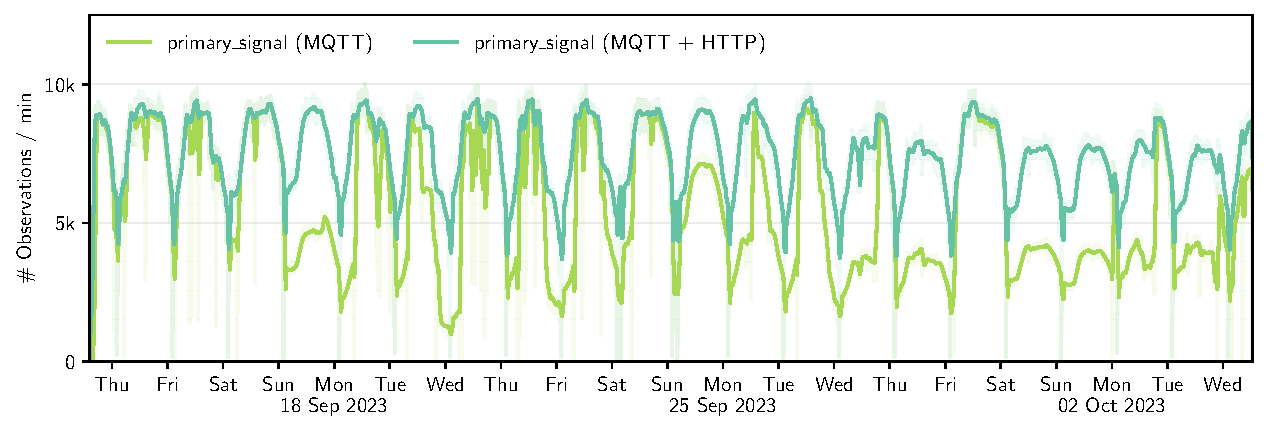
\includegraphics[width=\linewidth]{images/adaptiveness-mqtt-http.pdf}
    \caption{Supplementation of recorded MQTT observations through HTTP interface.}\label{fig:adaptiveness-mqtt-http}
\end{figure}

\Cref{fig:adaptiveness-mqtt-http} demonstrates that this approach effectively minimizes data losses. On multiple days, approximately half of all recorded observations were supplemented by the HTTP interface because they were lost preliminarily via MQTT. However, in the week around October 2, 2023, another issue arose, reducing the overall quantity of observations despite supplementation via HTTP. Therefore, it must be assumed that at least a small portion of the actual traffic light states could not be recorded.

The detection of faulty cycles, also implemented in the prediction service, was utilized for problem identification. Out of approximately 424 million reconstructed cycles, 13.8 million cycles were discarded. Here, 90\% of faulty cycles are distributed across 10\% of the connections. By examining the faulty connections on the map, one of the known faulty traffic controllers could be identified as the cause.

It is likely that only a subordinate part of faulty cycles was detected in this process. 35\% of the available traffic lights in Hamburg, according to the recorded data, switch only between red and green, making it impossible to identify missing phases using the established error detection. However, for 42\% of the traffic lights, the detection should have worked well, as it was determined that they switch in the order of green-amber-red-redamber. The remaining traffic lights switch between other colors, such as green and dark, represented by \texttt{primary\_signal} Observations with \texttt{result = 0}. However, these other patterns each represent only roughly 1\% or significantly fewer of the recorded cycles. Thus, these more exotic switching schemes were not excluded from the analyses in favor of a more complete perspective since no substantial effect on the interpretability of our metrics is expected.

In conclusion, we cannot completely eliminate all errors, but they seem to be present only to a minor extent. It is expected that isolated recording errors will be overshadowed by the mass of valid data. However, it is important to note for subsequent analyses that recording errors may have occurred, e.g., missing cycle observations leading to multiplied cycle lengths. Accordingly, we will use statistics for evaluation that are robust to outliers.

\begin{figure}[t]
    \centering
    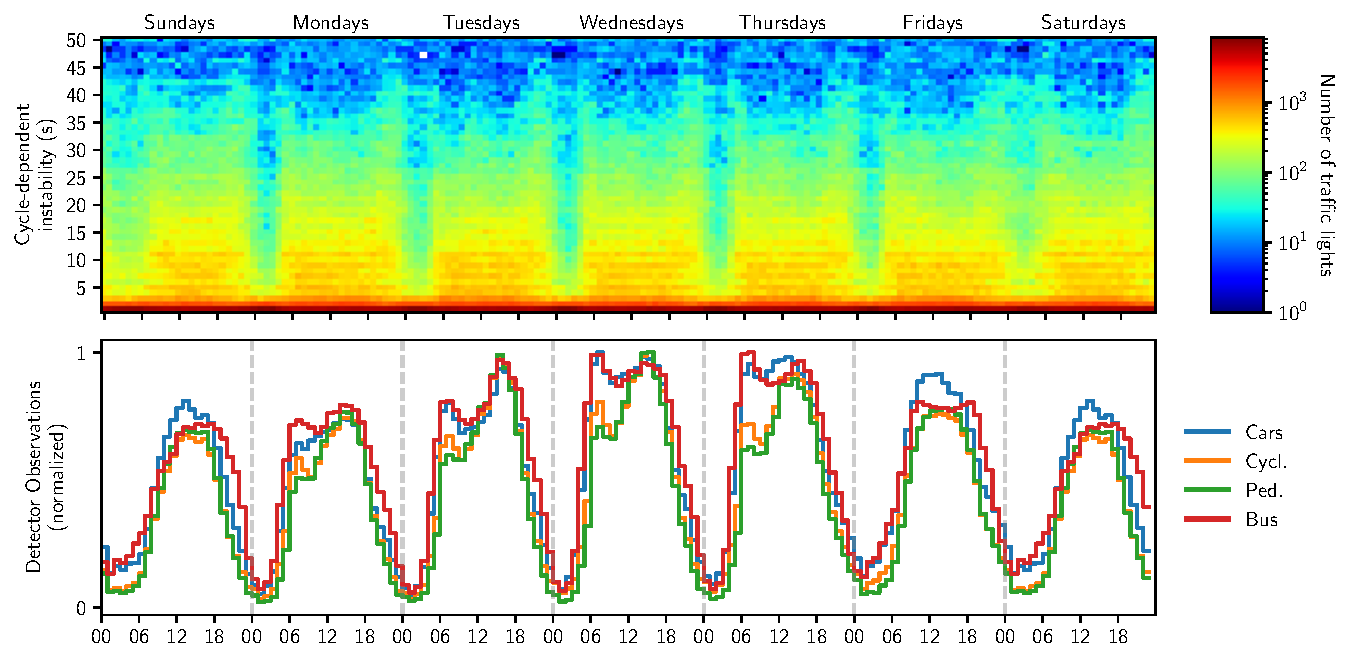
\includegraphics[width=\linewidth]{images/predictability-week-heatmap.pdf}
    \caption{Measured traffic light instability over weekdays in relation to the measured traffic volume.}\label{fig:adaptiveness-weekdays-distance}
\end{figure}

The first chart displayed in \Cref{fig:adaptiveness-weekdays-distance} looks at the relation between traffic light predictability and daytime. To get an insight into which hours and days during the week the predictability is highest, we calculate the cycle-dependent instability that provides a scalar value of the adaptiveness. We calculate this metric between all cycles within each hour distributed across each weekday in the four recorded weeks. The extracted week table forms the basis for examining trends across all traffic lights.

We use the median of the cycle-dependent instability for each hour and for each traffic light instead of the mean because it the mean would be affected by outliers due to missing cycle time observations. The median is more robust against such outliers. Additionally, we calculate the interquartile range (IQR) of the first and third quartiles of the metric distribution. The IQR provides a similar insight into the distribution of adaptability within the respective hour, like the dispersion measure, but is also statistically more robust against outliers. The information is presented along with the normalized frequencies of recorded bus requests (bus observations) as well as cars, bikes, and pedestrians (detector observations) to compare the measured instability to the measured traffic volume.

As a result, we observe that instability correlates, as expected, with traffic volume. While the instability is at its lowest during the night, it rises rapidly during the morning traffic surge. However, it then remains relatively constant after reaching an upper bound until the evening before decreasing again. The plateaus of instability during daytime indicate that there may be limits to the instability even in the presence of increasing traffic. 

Another significant observation is that most traffic lights reside within a low range of instability. Measured across all traffic lights, the median of the distance metric ranges between 0 and 3 seconds depending on the daytime. Interpreting the interquartile range (IQR): at least 25\% of all traffic lights exhibit no persistent instability in the median, and at least 75\% of all traffic lights in the median operate with a maximum instability of 15 seconds. In general, these results correspond with the observation that the designed prediction algorithm is able to accurately predict Hamburg's traffic lights in a large proportion of cases. Nonetheless, they again underline that traffic lights equipped with traffic-adaptive capabilities do not necessarily have to express a corresponding adaptive behavior or are at least highly limited in their adaptiveness.

\begin{figure}[t]
    \centering
    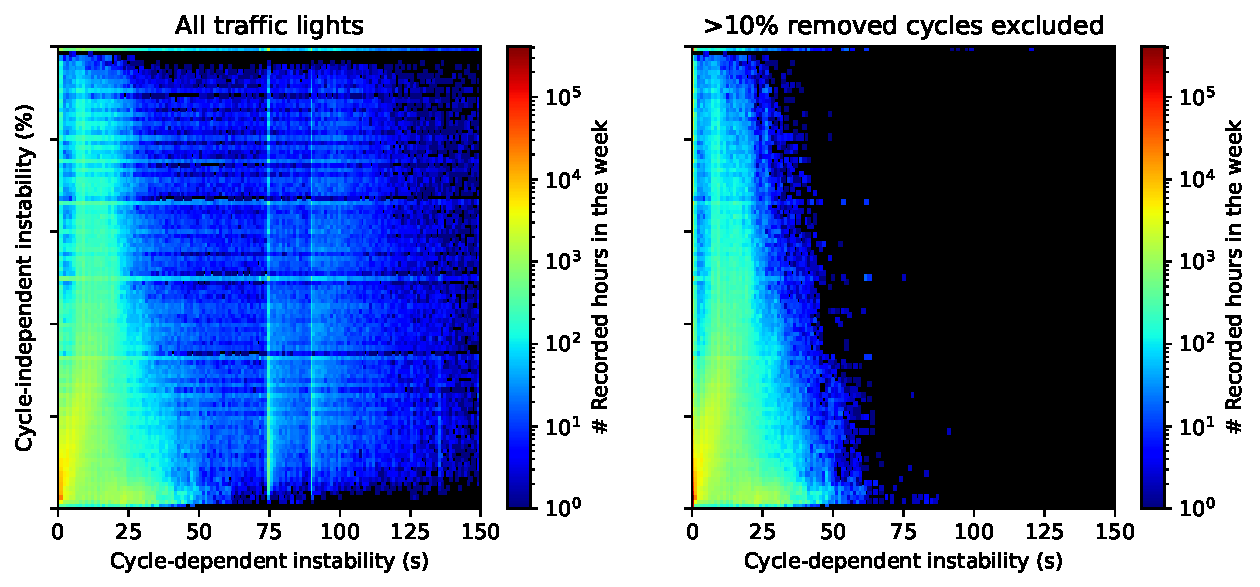
\includegraphics[width=\linewidth]{images/predictability-heatmap.pdf}
    \caption{.}\label{fig:predictability-heatmap}
\end{figure}

A more conjugated perspective on the instability is given in \Cref{fig:predictability-heatmap} in which the cycle-dependent metric is set in relation to the cycle-independent metric. The visualization employs hourly granularity, allowing us to accurately capture transitioning traffic lights between adaptive and non-adaptive programs. For instance, a traffic light that switches between adaptive and non-adaptive modes 50\% of the time is represented with both adaptive and non-adaptive hours in the diagram. Consequently, the color scale's maximum value exceeds $10^5$ measured hours on a histogram element, in which one traffic light typically encompasses a few hundred values.

It is evident from this visualization again that many traffic lights exhibit low persistent adaptivity. Out of the evaluated 2,793,786 traffic light hours, 43\% (1,206,817) have a cycle-dependent instability of less than 5 seconds and a cycle-independent instability of less than 10\%. Traffic lights with more green phases tend to have lower cycle-independent instability than those with fewer green phases. Nevertheless, this visualization shows again that a large proportion of traffic lights reside within a relatively stable regime.

Outside of the large stable proportion of traffic lights, there are three other notable observations. First, a vertical line at cycle-dependent instability = 0 indicates traffic lights that only occasionally switch to green. Approximately 9\% (245,379) of recorded traffic light hours are associable with this behavior: they have a median cycle-dependent instability of 0 seconds but a cycle-independent instability higher than 10\%. 

Second, the horizontal line at cycle-independent instability = 1 suggests cases where cycles are highly unstable or non-green signal colors alternate unevenly, such as black-amber. This is likely a measurement artifact and does not necessarily indicate a causal relationship with the actual switching behavior. Finally, background noise recorded above 50 seconds of cycle-dependent instability, especially visible vertical line artifacts, generally suggests faulty data in these areas. Excluding traffic lights with more than 10\% of cycles discarded due to detected errors largely eliminates these error patterns from the visualization, confirming this interpretation.

\begin{figure}[t]
    \centering
    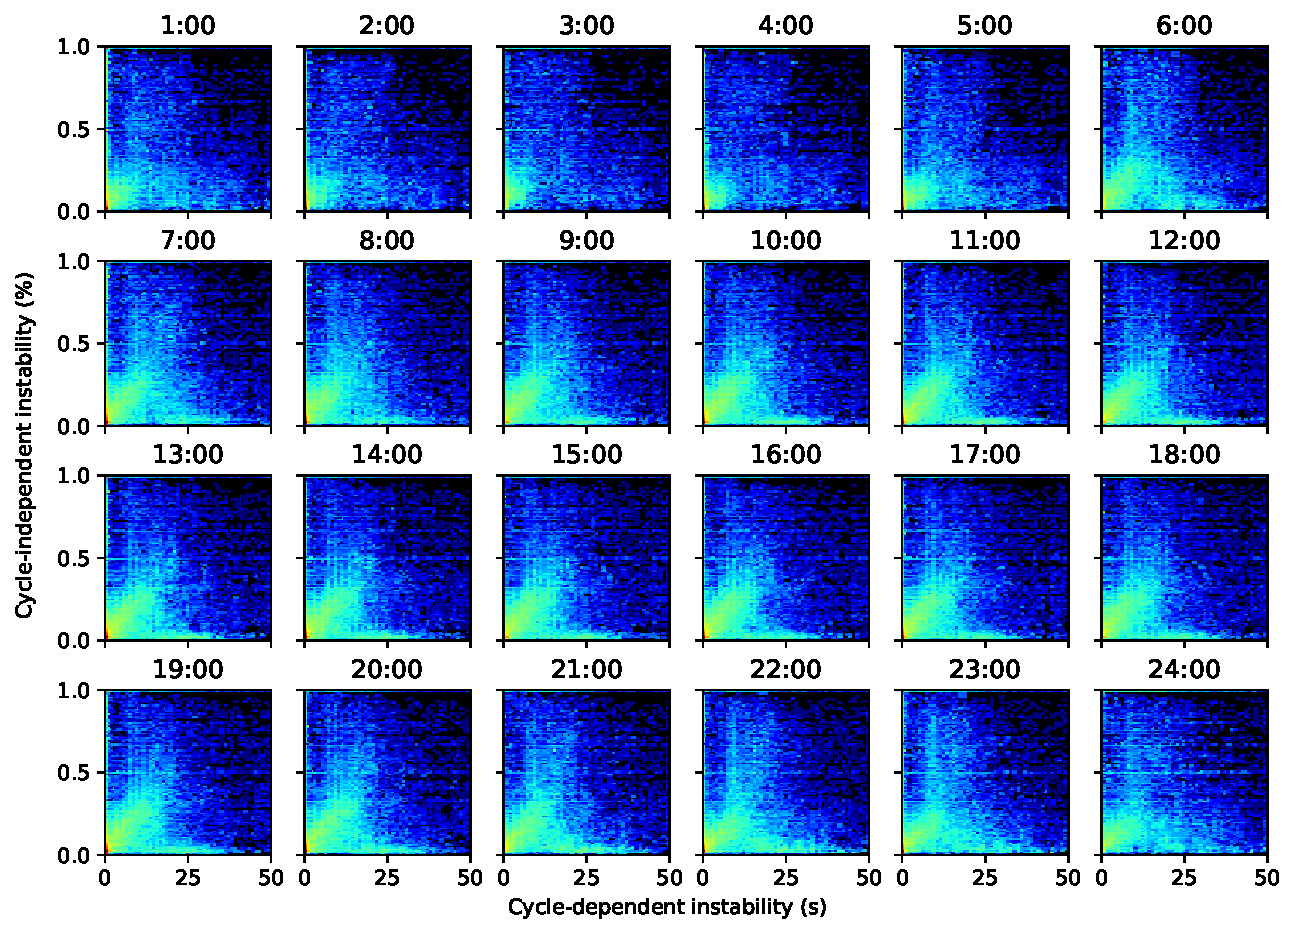
\includegraphics[width=\linewidth]{images/predictability-heatmap-hourly.pdf}
    \caption{.}\label{fig:predictability-heatmap-hourly}
\end{figure}

Some recorded hours exhibit low cycle-independent instability but high cycle-dependent instability. This suggests the presence of step patterns but may also result from data errors such as missing cycle observations.

\Cref{fig:predictability-heatmap-hourly} further dissects the relationship between cycle-dependent and cycle-independent instability throughout the day. When comparing hours, a distinct difference is observed before 6 AM and after 6 AM, persisting until around 11 PM. The increase in adaptiveness during the day aligns with the moment when adaptivity, as shown in \Cref{fig:adaptiveness-weekdays-distance}, starts to increase. 

Interestingly, although many traffic lights experience an increased cycle-independent instability during that period, there are also some traffic lights that express a decreased cycle-independent instability while having a high cycle-dependent instability. One potential interpretation is that, during the plateau of instability during the day, these traffic lights are permanently triggered by traffic participants, resulting in a relatively stable period of green phases and a step-like pattern unaligned with the cycle time.

However, this interpretation should be handled with caution since 6 AM is also the time when, according to \Cref{fig:monitoring-7-days}, data failures become more prevalent. Examining case studies of this period helps us understand whether the interpretation of increased step patterns during the day is valid or whether the observed relation is solely induced by data errors.

\begin{figure}[htbp]
\centering 
\begin{tabular}{|c|c|c|}
\hline
& \footnotesize{\textbf{Cycle-dependent instability <5s}} & \footnotesize{\textbf{Cycle-dependent instability >25s}} \\
\hline
\rotatebox{90}{\footnotesize{\textbf{\hspace{0.18cm} Cycle-independent instability >90\%}}} & B 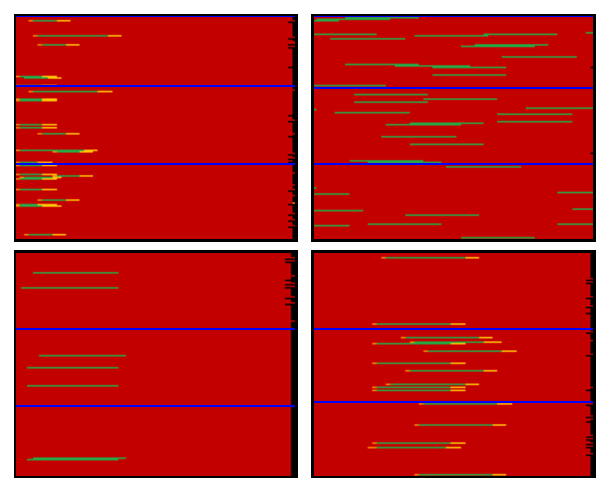
\includegraphics[width=0.42\linewidth]{images/predictability-rw-example-top_left.pdf} & D 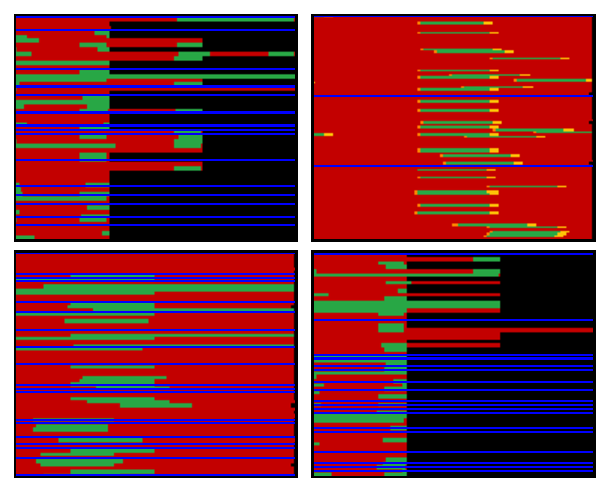
\includegraphics[width=0.42\linewidth]{images/predictability-rw-example-top_right.pdf} \\
\hline
\rotatebox{90}{\footnotesize{\textbf{\hspace{0.18cm} Cycle-independent instability <10\%}}} & A 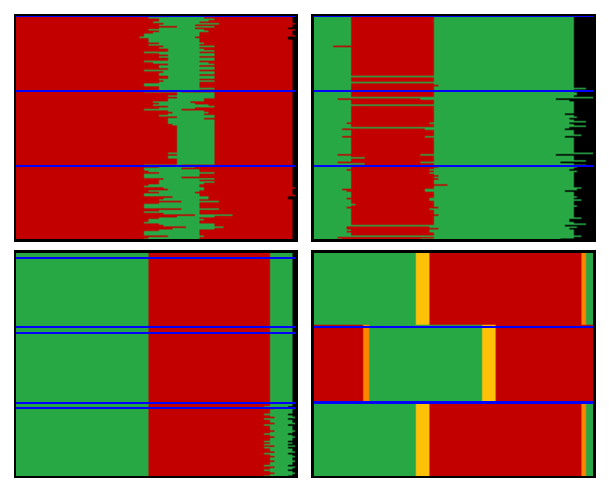
\includegraphics[width=0.42\linewidth]{images/predictability-rw-example-bottom_left.pdf} & C 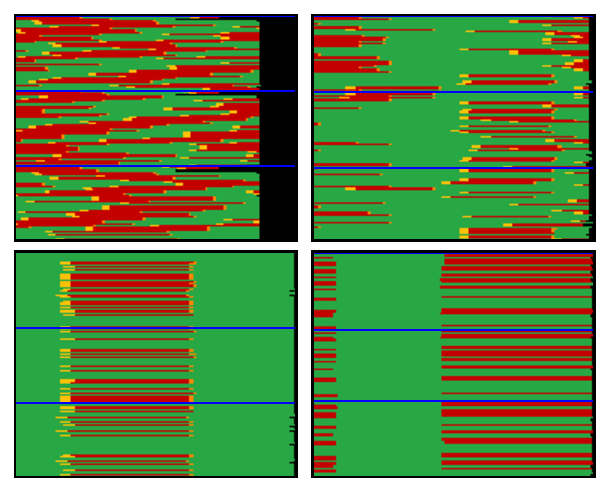
\includegraphics[width=0.42\linewidth]{images/predictability-rw-example-bottom_right.pdf} \\
\hline
\end{tabular}
\caption{.}
\label{fig:types-of-instability}
\end{figure}

Figure \ref{fig:types-of-instability} illustrates randomly chosen examples for each section of the instability diagram. Seen in this visualization are also examples from case C, towards which some traffic lights drift throughout the day. The observed patterns indeed indicate some fully traffic-dependent traffic lights triggered very frequently. However, based on the random sample, it can be inferred that such patterns are generally rare. Overall, most patterns, as described by Protschky et al. (2014) \cite{protschky_extensive_2014}, appear to be synchronized with the cycle length in this range.

Data errors can not be seen as frequently as expected for case C. Instead, a substantial part of examples in this region are traffic lights frequently switching between two stages. Although the switching pattern within each stage is stable and aligned with the cycle, the median of cycle-dependent instability is high due to the frequent switching between both stages. As a consequence, programs located in the lower right of the diagram are unexpectedly well predictable, at least for the secure recurring green phase, even with the probabilistic approach. Step patterns seem to be less prevalent, even for traffic lights measured in the lower right of the diagram.

In category D, as expected, there are initially traffic lights with strong adaptability. Surprisingly, this area also contains traffic lights that occasionally switch at a recurring time. More frequently, however, there are traffic lights with data errors. Blue lines indicate cycles that are discarded more often due to detected faulty switching behavior. Specifically, cycle observations are frequently missing, resulting in the cycle length doubling or tripling. Overall, it can be observed that many traffic lights measured in the upper right have a high data error rate. Nevertheless, assuming perfect data transmission, the predictability of these traffic lights is likely to be relatively poor based on the observed patterns in these case studies.

In conclusion, even with increased cycle-independent and cycle-dependent instability, partially stable patterns can still be measured, while problematic traffic lights are less common. Therefore, the forecasting situation can be considered relatively favorable.

\begin{figure}[t]
    \centering
    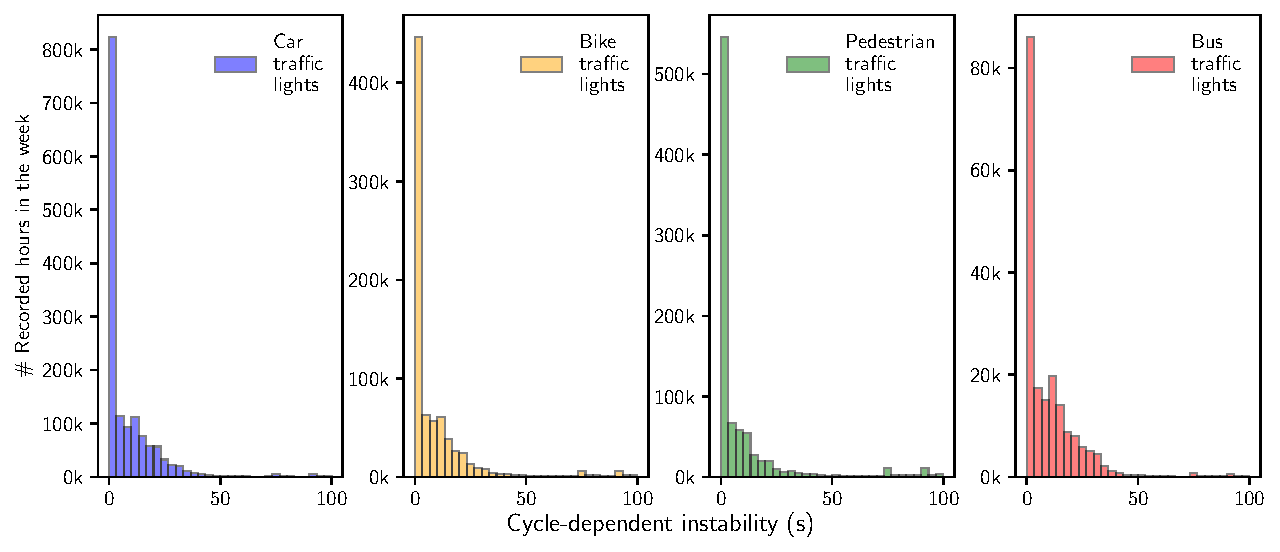
\includegraphics[width=\linewidth]{images/predictability-by-lanes.pdf}
    \caption{.}\label{fig:predictability-by-lanes}
\end{figure}
\begin{figure}[t]
    \centering
    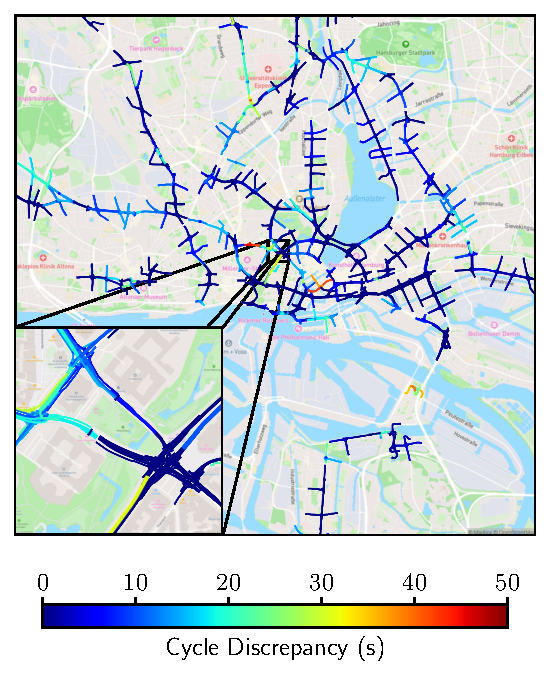
\includegraphics[width=\linewidth]{images/predictability-map.pdf}
    \caption{.}\label{fig:predictability-map}
\end{figure}

Finally, let's examine the distribution of instability across individual modes of transportation and the spatial distribution. As depicted in \ref{fig:predictability-by-lanes}, it is noteworthy that there are almost no differences in instability among different modes of transportation. Once again, the pattern emerges that traffic lights experience little to no persistent instability for the majority of the time. Overall, this implies that the predictability situation is similarly favorable for all modes of transportation.

One possible explanation for this uniformity is that traffic lights for different modes of transportation may be interconnected, leading them to exhibit similar levels of instability. This relationship is further illustrated on the map in \ref{fig:predictability-map}. The visualization demonstrates that instability often depends on the intersection. If individual traffic lights at a given intersection exhibit high instability, there is a significant chance that this behavior is mirrored in other traffic lights at the same intersection.

While the traffic light switching behavior is generally stable at most intersections, there are occasional intersections with higher instability. These intersections would be sensible focal points for testing a more complex prediction methodology.

\begin{Summary}[Summary of Results]

\end{Summary}

\section{Conclusions}
